% Autoren: Ursprüngliche Version von Eike Thaden, modifiziert von René Schumann und Andreas Lattner, modifiziert von Markus Strobel

\documentclass[
	a4paper,
	hidelinks,
	12pt,
	headsepline,
	numbers=noenddot,
	bibliography=totoc,
	index=totoc,
	fleqn,
	DIVcalc,
	headings=normal
	]{scrreprt}
% Standard-Dokument mit
%   Papierformat A4
%   Binderand 5 mmx
%   Schrift 12-Punkt
%   Linie unter der Kopfzeile
%   Nummern ohne Punkt am Ende
%   Literaturverzeichnis mit Nummer im Inhaltsverzeichnis
%   Index mit Nummer im Inhaltsverzeichnis
%   Formeln werden linksbündig statt zentriert angeordnet
%   Berechne automatisch gute Werte für DIV
%		Etwas kleinere Überschriften

% Fonts etc:
%   8-Bit-Fonts
\usepackage[T1]{fontenc}

% Schriftart
\usepackage{helvet}
%\usepackage{arial}

%damit die pdf kommentiert werden kann
\usepackage{pdfcomment}

% Tables
\usepackage{tabularx}
\usepackage{multirow}
\usepackage{colortbl}
\usepackage{booktabs}

\newcommand*{\tabbox}[2][t]{% 
   \vspace{-5pt}\parbox[#1][2.5\baselineskip]{0cm}{#2}}


%Binderand- und Seitenrandeinstellungen
\typearea[20mm]{15}

%   zusätzliche Symbole
\usepackage{textcomp,latexsym}

%   Latin1-Umlaute in der Eingabe
%\usepackage[latin1]{inputenc}
\usepackage[utf8]{inputenc}

% neu deutsche Rechtschreibung
\usepackage[ngerman]{babel}

% für die aktuelle Zeit
\usepackage{scrtime}

%für Definitionen, Theoreme u.Ä.
\usepackage{theorem}
%\theoremstyle{break}
\newtheorem{Def}{Definition}


% Web-Adressen auch mit T1-Encoding
%\usepackage[T1]{url}

% und in tt-Font
%\urlstyle{tt}

% zuverlässige Bildpositionierung
\usepackage{float}
% Beispiel
%\begin{figure}[H]
%  \centering
%\fbox{
%    \includegraphics[scale=0.35]{images/bildname}
%}
%  \caption{blabla}
%  \label{bla}
%\end{figure}

% Grafik
\usepackage[pdftex]{graphicx}

% Zur Einbindung von PDFs		
\usepackage{pdfpages}


 % Tikz Package for Drawing 
\usepackage{tikz}
% Tikz Node Positioning
\usetikzlibrary{positioning}
\usetikzlibrary{datavisualization} % LATEX and plain TEX
\usetikzlibrary[datavisualization] % ConTEXt
\usetikzlibrary{datavisualization.formats.functions}


% Mathematik: wer's braucht, sollte folgende Zeilen verwenden:
\usepackage{amsfonts}	
\usepackage{amsmath}
\usepackage{amssymb}

%Für das Setzen von Algorithmen
% Algorithm/Algorithmic-Umgebung für Algorithmen
%\usepackage{include/algorithm}
%\usepackage{include/algorithmic}

%\usepackage{listings}
%\lstset{
%	numbers=left,
%	numberstyle=\tiny,
%	numbersep=5pt,
%	basicstyle=\scriptsize,
%	breaklines = true
%}


% for quotation of source code
\usepackage{listings}
\usepackage{color}

\definecolor{dkgreen}{rgb}{0,0.6,0}
\definecolor{gray}{rgb}{0.5,0.5,0.5}
\definecolor{mauve}{rgb}{0.58,0,0.82}

\definecolor{red}{rgb}{1.0,0,0}

\definecolor{semicolor}{rgb}{0.84,.95,0.73}
\definecolor{hitcolor}{rgb}{0.57,.81,0.31}

\lstset{
  frame=single,
  frameround=ffff,
%  frameround=tttt,
  language=C++,
%  language=Java,
  aboveskip=3mm,
  belowskip=3mm,
  showstringspaces=false,
  columns=flexible,
  basicstyle={\small\ttfamily},
  numbers=none,
  numberstyle=\tiny\color{gray},
  keywordstyle=\color{blue},
  commentstyle=\color{dkgreen},
  stringstyle=\color{mauve},
  breaklines=true,
  breakatwhitespace=true,
  tabsize=4,
  captionpos=b
}





%% Hyperref erzeugt Hyperlinks in PDF-Dokumenten und erlaubt das
%% Setzen bestimmter Attribute
%\usepackage[
%% Titel der Arbeit
%pdftitle={InsertTitleHere},

%% Autor der Arbeit
%pdfauthor={Markus Strobel},

%% Art der Arbeit
%pdfsubject=[Masterarbeit]{hyperref}

% Wer's braucht: Verwende einen Index	
% Verwendung im Text: \index{Stichwort}
%\usepackage{makeidx}

% fette Seitenzahlen im index für die Hauptreferenz ermöglichen
% Verwendung: \index{Stichwort|ibf}
\newcommand{\ibf}[1]{{\bfseries #1}}

% Wer's hübscher findet: Numerierung von Formeln nicht mit
% Kapitelnummer.Formelnummer, sondern nur mit Formelnummer
%\renewcommand{\theequation}{\arabic{equation}}

% eine Randnote für fehlende Teile
\newcommand{\fehlt}[1]{(\marginpar[\hfill!$\longrightarrow$]{$\longleftarrow$!}Hier fehlt \emph{#1})}

% Keinen Einzug bei neuen Absätzen
 \setlength{\parindent}{0ex}

% Abstand zweier Listenelemente kleiner
\setlength{\itemsep}{0ex plus0.2ex}

% Benutze bei der Numerierung von Gleichungen "Kapitelnummer.Gleichungsnummer"
\renewcommand{\theequation}{\thechapter.\arabic{equation}}

% Abkuerzungsverzeichnis
\usepackage[printonlyused]{acronym}

% konfigurierbarer Zeilenabstand
\usepackage{setspace}





\pagenumbering{roman} 
% AB HIER GEHT ES LOS


% Angaben für das Titelblatt
\titlehead{
  \begin{center}
  
\includegraphics[scale=0.075]{images/Goethe-Logo_sw.png}\\ \vspace{0.1cm}

  {\scshape Fachbereich 12 -- Informatik und Mathematik}\\
  {\scshape Institut für Informatik}
	%\vspace{0.5cm}
  \end{center}				
}

\singlespacing
% Art der Arbeit	
\subject{Masterarbeit}
% Tite
\title{\normalsize{Monkey Brains Island - \\Eine BCI-Erweiterung für eine Point and Click Engine}}
\begin{titlepage}
% Autor
\author {
%\normalsize{			\textbf{Author}									} \\
\normalsize{			\textbf{Markus Strobel}									} \\
\normalsize{			Matrikelnummer: 3545258								}\\
\normalsize{			Frankfurt am Main, den \today 					}\\\\
\footnotesize{ 		\textbf{Betreuer}									} \\
\footnotesize{ 		Prof. Dr.-Ing. Detlef Krömker							} \\
\footnotesize{		Dipl. Inf. Matthias Pfeiffer								} \\\\
%\footnotesize{		\textbf{Erst- und Zweitgutachter}							}\\
%\footnotesize{		Prof. Dr-Ing. Detlef Krömker 							}\\
%\footnotesize{		Dr. Karsten Tolle									}
}


% Datum	
\date{
%\normalsize{		Frankfurt am Main, eingereicht am \today 				} 
%\normalsize{		Frankfurt am Main, den \today 				} 
%\vspace{0.2cm}
}


\end{titlepage}

% Rückseite des Titelblatts: Wann gesetzt?
% \lowertitleback{\small Gesetzt am \today{} um \thistime{} Uhr mit {\LaTeX}.}


% Erstelle den Index (nur benutzen, falls ein Index verwendet wird!)
\onehalfspacing
\makeindex
% Und hier geht es los
\begin{document}

	

    % Titelblatt
    \maketitle	




    % Eidesstattliche Erklärung
    \pagebreak
\begin{center}
\vspace{1cm}
\textbf{Erklärung gemäß Master-Ordnung 2008 §24 Abs. 12}
\vspace{1cm}

\end{center}

Hiermit bestätige ich, dass ich die vorliegende Arbeit selbstständig verfasst habe und keine anderen Quellen oder Hilfsmittel als die in dieser Arbeit angegebenen verwendet habe.\\
\vspace{2cm}


% \small {Frankfurt am Main, den \today }
% \vspace{-0.4cm} \\
\rule{0.45\textwidth}{0.4pt}
\hspace{1cm} 
\rule{0.45\textwidth}{0.4pt} 
\\
Ort, Datum \hspace{6cm} Unterschrift


    % Zusammenfassung / Abstract
     \chapter*{Zusammenfassung}

Die vorliegende Arbeit befasst sich mit der Realisierung einer \acs{BCI}-Erweiterung für eine Point\&Click Engine.
Es wird der Frage nachgegangen, welche \acs{BCI}-Paradigmen für diesen Zweck geeignet und realisierbar sind.
Aus dieser Frage ergeben sich daher mehrere Möglichkeiten zur Darstellung visueller Stimuli, dessen nähere Auswahl anhand des Point\&Click-Eingabeparadigmas erfolgt.
Zusätzlich werden verschiedene Szenarien für die Präsentation dieser Stimuli betrachtet, sowie deren Vor- und Nachteile spezifiziert.

Die Erstellung des Konzepts erfordert zudem die Recherche und Auswahl einer quell\-offenen Point\&Click Engine, sowie einer ebenso frei verfügbaren BCI-Software für die Verarbeitung und Auswertung der EEG-Daten.
Im Konzept werden die verschiedenen Komponenten detailliert betrachtet und miteinander verknüpft, sowie die Interprozesskommunikation definiert.\\
Während der Implementierung wird infolge des Konzepts ein Plugin für die Point\&\-Click Engine \textit{Adventure Game Studio} und eine Modifikation basierend auf dem P300-Speller des \textit{BCI2000}-Frameworks entwickelt.
Das Plugin erweitert die Engine um zusätzliche Funktionen und ermöglicht die Definition beliebiger Speller-Matrizen.
Beide Komponenten kommunizieren Parameter und Ergebnis und ermöglichen durch abwechselnde Aktivität den Spielfluss.\\
Im Anschluss an die Implementierung wird eigens ein Test-Spiel konzipiert und entwickelt, sowie ein Evaluations-Konzept für die Verifikation der Erweiterung ausgearbeitet.
Die Tests sehen den Vergleich zwischen den Ergebnissen des \textit{BCI2000}-P300-Spellers und des modifizierten P300-Spellers vor und sollen die Korrektheit der Erweiterung verifizieren.
Darüberhinaus beinhalten die User-Tests mehrere Fragebögen und ermitteln die subjektive Belastung des Anwenders mittels NASA TLX.
Abschließend werden die gesammelten Ergebnisse angemessen visualisiert und zeigen, dass die Steuerung eines Point\&Click-Adventures mit der entwickelten \acs{BCI}-Erweiterung möglich ist.\\


     \pagenumbering{arabic}

    % Inhaltsverzeichnis
    \setcounter{secnumdepth}{1}
    \tableofcontents

    \singlespacing
  % Abkuerzungsverzeichnis
    
\section*{Abkürzungsverzeichnis}

\begin{acronym}[Bash]
 \acro{AEnima}{Graphical User Interface Module des BCI++ Frameworks} 
 \acro{AGS}{Adventure Game Studio}
 \acro{BCI}{Brain Computer Interface}
 \acro{BCI2000}{Eine Quelloffene Software-Platform für Brain Computer Interfaces}
 \acro{BGRA}{Repräsentation der Farbkanäle eines Bildes in Blau-Grün-Rot-Alpha}
 
 \acro{EEG}{Elektroenzephalograpie} 
 \acro{EMG}{Elektromyographie}
 \acro{EOG}{Elektrookulographie}
 
 \acro{GUI}{Graphische Benutzeroberfläche (Graphical User Interface)}
 
 \acro{fMRT}{funktionelle Magnetresonanztomographie} 
 
 \acro{HIM}{Hardware Interface Module} 

 \acro{LIS}{Locked-In-Syndrom} 
 \acro{MEG}{Magnetoenzephalographie}
 
 
 \acro{NASA-TLX}{NASA Task Load Index}

 \acro{P300 ERP}{P300 \textit{"'Event-Related Potential"'}}
 \acro{RGBA}{Repräsentation der Farbkanäle eines Bildes in Rot-Grün-Blau-Alpha}

 \acro{SMR}{Sensomotorischer Rhythmus}
 \acro{SSEP}{Steady-State Evoked Potentials}
 \acro{SWLDA}{schrittweise lineare Diskriminanzanalyse}
 
 \acro{TOBI}{Tools for Brain-Computer Interfaces}



\end{acronym}
    \onehalfspacing

    % der eigentliche Text
    % Kapitelübersicht
    % 1) Einleitung - Problembeschreibung, Vorstellung der Arbeit, Übersicht über die Arbeit (wo steht was?)
	\chapter{Einleitung}

\section{Motivation}

Die Fähigkeit etwas mit seinen Gedanken zu steuern, ist schon seit langem ein erstrebenswerter Traum der Menschen.
So leicht es in Science-Fiction Büchern erscheinen mag, ist es in der Realität eine nicht zu unterschätzende Herausforderung.
Dennoch handelt es sich hierbei um ein interessantes Themengebiet, das noch am Anfang seiner Entwicklung steht.
Der aktuelle Forschungsstand bedeutet für durchschnittliche Menschen noch nicht viel, doch für einige Menschen mit motorischen Störungen können selbst die kleinsten Entwicklungen in diesem Bereich enorme Möglichkeiten bieten.
Die Forschung der vergangenen Jahrzehnte brachten einige Paradigmen im Bereich der Gehirn-Computer-Schnittstellen hervor.
Seitdem wurde eine Vielzahl von Anwendungen entwickelt, um diesen Menschen eine
Möglichkeit zu geben sich auszudrücken und so ihr Leben zu erleichtern.
Diese Masterarbeit soll in diesem Kontext eine Erweiterung für eine Spiele Engine entwickeln, sodass Erzeugnisse dieser Engine mit eine Gehirn-Computer-Schnittstelle gespielt werden können.\\







\section{Beschreibung der Aufgabenstellung}

Gegenstand dieser Arbeit wird es sein, Konzept und Implementierung einer \acs{BCI}-Erweiterung für eine Point\&\-Click Spiele Engine auszuarbeiten und diese zu realisieren.
Zu diesem Zweck ist es erforderlich, dass mögliche Hard- und Softwarekomponenten untersucht und ausgewählt werden.
Dies erfordert insbesondere die Kopplung der \acs{BCI}-Software und der Spiele Engine in geeigneter Weise.
Des Weiteren wird eine Untersuchung und Auswahl der \acs{BCI}-Paradigmen benötigt, da diese maßgeblichen Einfluss auf die Implementierung der Erweiterung haben.


Abschließend müssen Tests konzipiert und durchgeführt werden, sodass eine Verifizierung der Erweiterung erfolgt und sichergestellt wird, dass die Aufgabe dieser Arbeit korrekt erfüllt wurde.\\





	
    % 2) Grundlagen - Was ist allgemein Wichtig?
	%\include{zeitplan} %kommt später wieder raus
	\chapter{Grundlagen}
In diesem Kapitel werden dem Leser die erforderlichen Grundkenntnisse für das Verständnis der vorliegenden Masterarbeit näher gebracht. \\




\section{Brain Computer Interface}

Ein \ac{BCI} ist eine Schnittstelle zwischen Gehirn und Computer, 
welche es ermöglicht Signale des Gehirns in verwertbare Informationen zu verwandeln.
Diese Informationen eröffnen dem zentralen Nervensystem, neben der neuromuskulären und der hormonellen, 
eine weitere Möglichkeit zur Kommunikation mit seiner Umwelt.

Dieser künstlich generierte Informationskanal kann genutzt werden, 
um verlorene oder eingeschränkte Fähigkeiten von Menschen mit motorischen Störungen in begrenzter Form wiederherzustellen.
Zusätzlich können diese Daten auch zur Verbesserung der Fähigkeiten gesunder Menschen beitragen \cite[S.3]{wolpaw2012braincomputer} 
oder in Abhängigkeit der gesammelten Daten könnte unterstützender Einfluss auf Hard- oder Software genommen werden.\\ \\
Die Aufzeichnung der Gehirnströme kann über invasive- oder nicht-invasive Methoden erfolgen.
Invasive Methoden zeichnen die Gehirnaktivität über Elektroden im Gehirn oder auf der Hirnhaut auf, 
während nicht-invasive Methoden die Signale indirekt über die Kopfhaut beziehen.
Die Messungen der Gehirnströme kann unter anderem über Magnetenze\-phalographie (\acs{MEG}), \ac{fMRT} oder \ac{EEG} \cite{berger2008braincomputer} erfolgen.

\pagebreak
\subsection{Elektroenzephalographie}
\vspace{0.3cm}
Die \acf{EEG} ist die am häufigsten verwendete Methodik zur Messung der Gehirnaktivität.
Bei ihr handelt es sich um eine nicht-invasive Messmethode wobei Elektroden auf der Kopfhaut platziert werden.
Für die Elektrodenplatzierung gibt es verschiedene international anerkannte Systeme, die je nach Anzahl und Position der Elektroden eine höhere Genauigkeit ermöglichen.
In Abbildung\footnote[1]{Bild-Quelle: \cite{Oostenvald2001}} \ref{electrodes} sind die Elektrodenpositionen gemäß des internationalen "`10-20-Systems"' \cite[S.370-375]{Jasp58} und des "`10-10-Systems"' dargestellt.
Die Kennzahl der Systeme gibt dabei Auskunft über den relativen Abstand der einzelnen Elektroden in Bezug zu Referenzpunkten auf der Kopfoberfläche.\\


\begin{figure}[h!]
\begin{center}
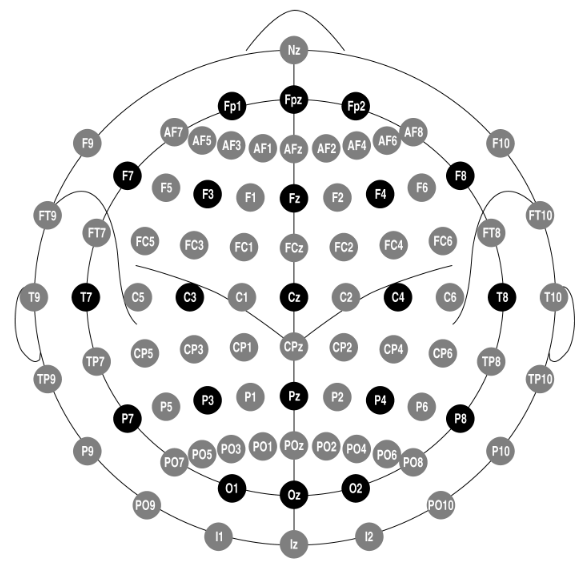
\includegraphics[scale=0.61]{images/1010.png}
\caption{Die Elektrodenpositionen des internationalen 10-20-Systems (schwarz) und des 10-10-Systems (schwarz und grau)}
\label{electrodes}
\end{center}
\end{figure}


Die Verwendung von \acs{EEG}'s ist deshalb vorteilhaft, da sie relativ kostengünstig und einfach einzusetzen sind.
Medizinische \acs{EEG}'s befinden sich überwiegend in speziell abgeschotteten Räumen, jedoch gibt es auch einfache zu handhabende tragbare Geräte, sodass eine hohe Verfügbarkeit besteht.
Allerdings existieren neben den Vorteilen auch Nachteile, da die Auflösung und Frequenzreichweite begrenzt ist und Artefakte durch Muskelaktivität oder Augenblinzeln entstehen können \cite{Graimann2010}.









\subsection{Oddball-Paradigma}
\vspace{0.3cm}

Das Oddball-Paradigma oder auch Zwei-Reiz-Diskriminationsparadigma \cite[S.9]{paehge2006verschiedenen} genannt, 
beschreibt eine besondere Charakteristik von Stimulus-Ereignissen, die in zwei Klassen unterteilt werden können.
Dabei existiert eine Klasse von häufigen und eine Klasse von seltenen Ereignissen. 
Jedes der seltenen und damit unerwarteten Ereignisse ist ein "`Oddball-Ereignis"'.\\



\subsection{P300 Ereigniskorreliertes Potential}
\vspace{0.3cm}

Im Zusammenhang mit einem "`Oddball-Ereignis"' steht in der Regel ein ereigniskorelliertes positives Potential.
Es tritt etwa 300ms nach dem auslösenden Ereignis auf. 
Die Latenzzeit kann jedoch zwischen 250ms und 750ms variieren, was von der nicht notwendigerweise bewussten Entscheidung abhängt, ob das Ereignis aufgetreten ist.\\

\begin{figure}[h!]
\begin{center}
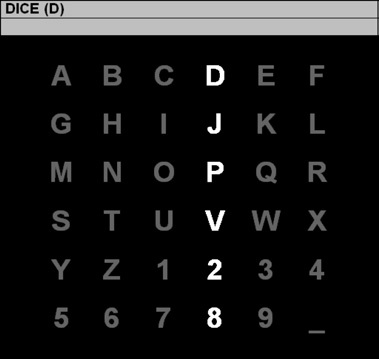
\includegraphics[scale=0.6]{images/P300Speller.jpg}
\caption{Die 6x6 Matrix eines P300 Spellers mit hervorgehobener Spalte}
\label{P300Speller}
\end{center}
\end{figure}

Basierend auf diesem \ac{P300 ERP} wurde 1988 von Farwell und Donchin \cite{FarwellDonchin1988} ein sogenannter \textit{"`P300 Speller"'} eingeführt. 
Dabei werden die Stimuli als Zeilen und Spalten einer Matrix zusammengefasst. 
Die Zeilen und Spalten der Matrix werden hierbei in zufälliger Reihenfolge kurz sichtbar hervorgehoben, wie in Abbildung\footnote[1]{Bild-Quelle: \cite[S.300]{P300SpellerCompare}} \ref{P300Speller} zu sehen ist. 
Der Benutzer sollte sich während dieser Prozedur auf das auszuwählende Feld konzentrieren. 
Sobald die Zeile bzw. Spalte des Zielfelds aufblitzt, wird ein \acs{P300 ERP} evoziert. 
Das Zielfeld ergibt sich anschließend aus Kombination der Zeilen und Spalten, die ein \acs{P300 ERP} ausgelöst haben.
Durch dieses Vorgehen ist es möglich für viele verschiedene Anwendungsmöglichkeiten "`Ja/Nein"'- bzw. "`Ziel/Nicht-Ziel"'-Antworten zu ermitteln.
Dieses Prinzip funktioniert bei allen Experimenten deren Ereignisse dem Oddball-Paradigma folgen \cite[S.215ff]{wolpaw2012braincomputer}.\\



\subsection{Emotiv EPOC}
\vspace{0.3cm}

Das Emotiv EPOC \cite{Emotiv2014} in Abbildung \ref{EmotivEPOC} ist ein für praktische Anwendungen entwickeltes, hochauflösendes und portables \acs{BCI}.
Es verwendet für die \acs{EEG}-Signalerfassung 16 Kanäle, wovon 2 als Referenz dienen.
Die Elektroden des Emotiv EPOC werden gemäß des internationalen "`10-20-System"' \cite[S.370-375]{Jasp58} an den Positionen 
AF3, F7, F3, FC5, T7, P7, O1, O2, P8, T8, FC6, F4, F8, AF4 platziert (Zu sehen in Abbildung\footnote[1]{Bilder-Quelle: \cite{Emotiv2014}}
\ref{EmotivMAP}). 
Die Genauigkeit kann allerdings durch individuelle Faktoren wie die Kopfgröße negativ beeinflusst werden, da die Elektrodenplatzierung des Emotiv EPOC auf eine Größe genormt ist.\\

\begin{figure}[ht]
\centering
\begin{minipage}[b]{0.45\linewidth}	
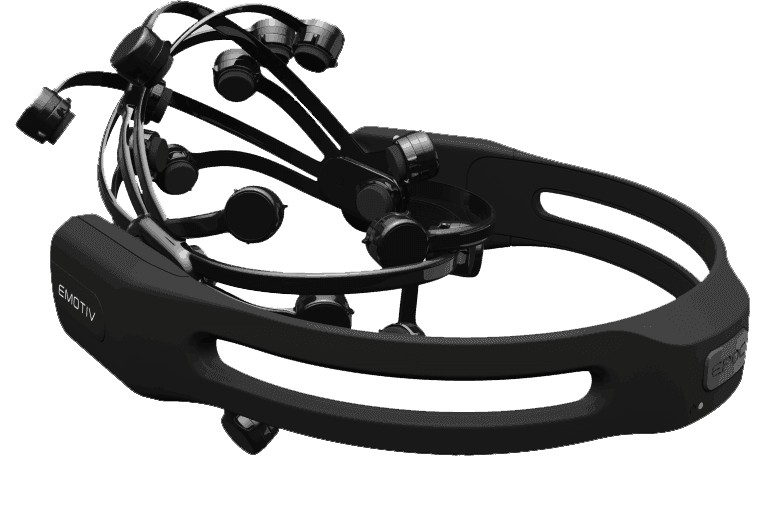
\includegraphics[scale=0.3]{images/emotivEpoc.png}
\caption{Das Emotiv EPOC \acs{BCI}}
\label{EmotivEPOC}
\end{minipage}
\quad
\begin{minipage}[b]{0.45\linewidth}
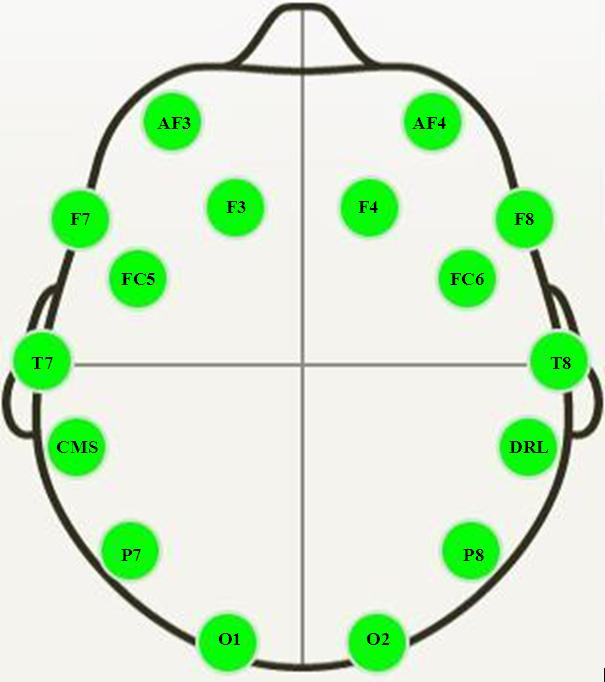
\includegraphics[scale=0.3]{images/emotivMap.jpg}
\caption{Die Elektroden des Emotiv EPOC}
\label{EmotivMAP}
\end{minipage}
\end{figure}








\pagebreak
\section{BCI2000}
\label{BCI2000}
Bei \acs{BCI2000} handelt es sich um eine quelloffene Software Plattform zur Verwendung von Brain-Computer-Interfaces. 
Sie wurde entwickelt, um ein leistungsfähiges und einfach zu erweiterndes \acs{BCI} Forschungs-Framework bereitzustellen.
Das Framework stellt viele Module zur Signalerfassung, -bearbeitung und -verwertung zur Verfügung. 
Insbesondere gibt es für viele \acs{BCI}'s entsprechende Module zur Signalerfassung.

Damit die Echtzeiterfassung der Daten gewährleistet werden kann, ist die Platform in C++ geschrieben.
Die Programmstruktur ist modular,
wie in Abbildung\footnote[1]{Bild-Quelle: \cite[S.39]{schalk2010practical}} \ref{BCI2000Design},
aus vier Teilen zusammengesetzt.
Das \textit{Operator}-Modul ist hierbei das Herzstück der Platform und je nach Notwendigkeit können die drei anderen Module ausgetauscht oder erweitert werden.\\

\begin{figure}[h!]
\begin{center}
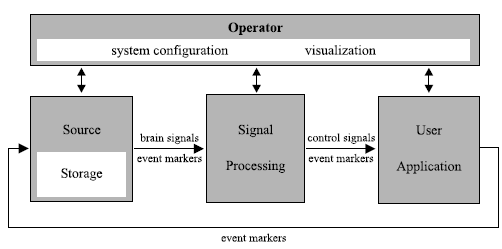
\includegraphics[scale=1]{images/BCI2000Design.png}
\caption{Eine vereinfachte Darstellung des Designs der \acs{BCI2000} Platform.}
\label{BCI2000Design}
\end{center}
\end{figure}

\begin{itemize}
\item Das \textit{Operator}-Modul: Dieses Modul steuert das Zusammenwirken aller vier Module.
\item Das \textit{Source}-Modul: Dieses Modul bezieht die \acs{EEG}-Signale und reicht sie an das \textit{Signal-Processing}-Modul weiter.
\item Das \textit{Signal-Processing}-Modul: Dieses Modul verarbeitet die erhaltenen Sig\-nale, extrahiert Merkmale und leitet diese als verwertbare Befehle weiter.
\item Das \textit{User-Application}-Modul: Dieses Modul empfängt die Befehle des \textit{Signal-Processing}-Modules
und benutzt diese zur Steuerung der Applikation oder des zugrunde liegenden Geräts. Des Weiteren steuert es die Präsentation der Stimuli und markiert diese im \textit{Source}-Modul, 
so dass eine Assoziation zwischen Stimuli und Signal möglich ist. \\
\end{itemize}

Die Architektur des \acs{BCI2000} ist so konzipiert, dass immer alle vier Module nacheinander ausgeführt werden müssen. 
Dabei fungiert das \textit{Operator}-Modul gewissermaßen als Server, bei dem sich die anderen drei Funktionsmodule anmelden. 
Die Interprozesskommunikation zwischen den vier Modulen geschieht mittels einem auf TCP/IP basierenden Protokolls \cite[s.38ff]{schalk2010practical},
worüber Signal- und Steuerinformationen, sowie globale Zustandvariablen kommuniziert werden können.
Die in der Abbildung dargestellten "`event markers"' zwischen dem \textit{User-Application}-Modul und dem \textit{\mbox{Source}}-Modul sind in diesem Zusammenhang besonders wichtig, 
da diese mit Hilfe einer Assoziationskarte die Zuordnung der einzelnen Stimuli und korrespondierender \acs{P300 ERP} ermöglichen.\\




\pagebreak
\section{Point\&Click}
Bei "`Point\&Click"' handelt es sich um ein Computerspiel-Genre, deren Spiele üblicherweise dem Eingabeparadigma der alleinigen Maussteuerung folgen \cite[Kapitel 11]{darby2013creating}.
Diese häufig auch "`Point\&Click-Adventures"' genannten Spiele, 
versetzen den Spieler in eine meist fiktive Welt und führen ihn durch eine dazugehörige Geschichte ein.
Solche Welten werden oft als einzelne Szenen oder Räume dargestellt, aber auch eine kontinuierliche Darstellung ist möglich.
Eine Szene ist für gewöhnlich ein Zimmer in einem Haus oder eine Landschaft in der Objekte, Charakter und Ereignisse integriert sind. 
Der Spieler erkundet die Szenen in aller Regel und muss oftmals Rätsel lösen, um im Spielfortschritt weiter voranzuschreiten.
Mit der Maus werden deshalb die zur Verfügung stehenden Aktionen ausgewählt, um anschießend das Ziel für diese zu bestimmen.\\
Gut durchdachte Spiele dieses Genre können durch ihre Rätsel sehr herausfordernd sein und die Aufmerksamkeit eines Spielers fördern.
Da bei klassischen Point\&Click-Spielen jedoch keine kontinuierliche Steuerung erfolgt, sind diese im allgemeinen langsamer als andere Spiele.
Einer der bekanntesten Ableger dieses Genres ist unter anderem die von LucasArts entwickelte "`The Secret of Monkey Island"'-Reihe von 1990, 
dargestellt in Abbildung\footnote[1]{Bild-Quelle: \cite{TSOMI90} } \ref{MonkeyIsland}. \\


\begin{figure}[h!]
\begin{center}
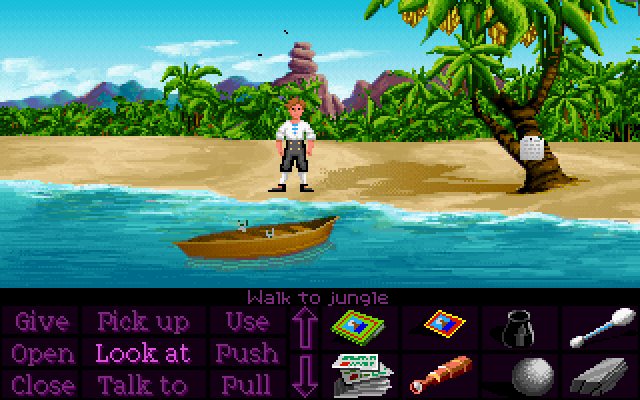
\includegraphics[scale=0.7]{images/monkeyIsland.png}
\caption{Eine Szene aus "`The Secret of Monkey Island"'}
\label{MonkeyIsland}
\end{center}
\end{figure}


\pagebreak
\section{Adventure Game Studio}
Das \ac{AGS}\footnote{Quelle: \cite{AGS2014}} 
ist eine quelloffene Point\&Click Spiele Engine, 
die in C++ geschrieben wurde und aus der eigentlichen Engine und einem dazugehörigen Editor besteht.
Zu Beginn dieser Masterarbeit lag die Engine in der Version 3.3 vor.
Sie besitzt eine umfangreiche Dokumentation und verfügt über ein Plugin-System zur einfachen Erweiterung der Engine und des Editors.
Das \acs{AGS} entwickelt sich, dank einer großen Gemeinschaft aus Engine- und Spieleentwicklern, kontinuierlich weiter.
Zudem existiert eine Vielzahl an Nutzern der daraus entstandenen Spiele.
Mit \acs{AGS} ist es möglich einfache Point\&Click-Adventures für Windows zu erstellen.
Eine Unterstützung für andere Betriebssysteme wie Linux oder MacOS soll es in zukünftigen Versionen geben.\\

Die Erstellung der Point\&Click-Adventures erfolgt im dazugehörigen Editor, einer einfach gehaltenen Entwicklungsumgebung, dessen Skript-Sprache auf Microsofts .NET Framework basiert.
Der Editor ermöglicht es Räume, Spielfiguren, Sounds und Grafiken innerhalb der Spiele zu erstellen und zu integrieren. 
Mit der integrierten Skript-Sprache können verschiedene Ereignisse ausgelöst und behandelt werden, um dem Spiel eine gewisse Dynamik zu verleihen.
Die Benutzeroberfläche eines Spiels kann vom Entwickler komplett individuell erstellt und auf die jeweiligen Bedürfnisse eines Spiels oder der Spieler angepasst werden.
Der Benutzer des Editors muss sich bei der Entwicklung eines Spiels keine Gedanken um Wegfindung oder Kameraführung machen.
Ebenso stellt die Engine Funktionen wie das Speichern und Laden von Spielständen bereit.
Diese müssen lediglich unter Verwendung der entsprechenden Befehle in die \ac{GUI} des Spiels integriert werden. \\
























	
    % 3) State of the Art - Was ist der aktuelle Stand der Technik. Wie wird aktuell das Problem gelöst?
	\chapter{State of the Art}
Innerhalb der nächsten Seiten wird die vorliegende Arbeit in den aktuellen Stand der Forschung eingeordnet.
Zu diesem Zweck werden aktuelle Arbeiten in Bezug auf die Anwendung und Anwendbarkeit von Brain Computer Interfaces vorgestellt.\\


\section{Aktuelle BCI-Anwendungen}
Die nachfolgenden Artikel beschreiben einige BCI-Anwendungen aktueller Forschungen unter Verwendung verschiedener Brain Computer Interfaces und den zugrunde liegenden Paradigmen.\\

\subsection{Brain Chess}
\vspace{0.3cm}
\label{chessconcept}
Schach ist ein rundenbasiertes Denkspiel, das durch seinen Aufbau und durch seinen vergleichweise langsamen Spielablauf hervorragend für eine \acs{BCI}-Steuerung geeignet ist.
"`Brain Chess – Playing Chess using Brain Computer Interface"' \cite[S.1-5]{BCIChess} befasst sich mit der Konzeption eines Schach-Spiels gesteuert durch ein Brain Computer Interface.
Vorranging werden in diesem Artikel Möglichkeiten erörtert, wie eine Steuerung einzelner Spielabschnitte unter Verwendung von Gehirnsignalen realisiert werden könnte.\\


Um eine Schachfigur auszuwählen muss zunächst mit Hilfe von einem Trainingsdatensatz, der spezifische Signalwert einer Figur ermittelt werden.
Dies wird durch ein "`Memory Card Game"' realisiert, so dass für jede Figur ein durchnittlicher Wert berechnet werden kann.
Anhand dieses Werts kann im Spielverlauf eindeutig bestimmt werden, welche Art von Figur ausgewählt wurde.\\

Sobald die Art der Figur bekannt ist, kann diese im Rahmen ihrer Möglichkeiten bewegt werden. 
Um die Bewegung zu realisieren wird eine Steuerung auf Basis von sensomotorischer Rhythmen (\acs{SMR}) vorgeschlagen, da dies die Unterscheidung einiger weniger Aktionen ermöglicht.
So können mit Hilfe der Vorstellung von Hand- oder Fußbewegungen die Bewegung der Schachfigur, wie in Abbildung\footnote[1]{Bild-Quelle: \cite[S.4]{BCIChess}} \ref{ChessPawn}, bestimmt werden.\\

\begin{figure}[h!]
\begin{center}
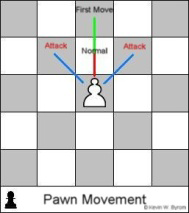
\includegraphics[scale=0.6]{images/ChessPawn.png}
\caption{Die vier Bewegungsmöglichkeiten eines Bauern, welche mit der Vorstellung von Hand- und Fußbewegungen assoziert werden können}
\label{ChessPawn}
\end{center}
\end{figure}

\begin{figure}[h!]
\begin{center}
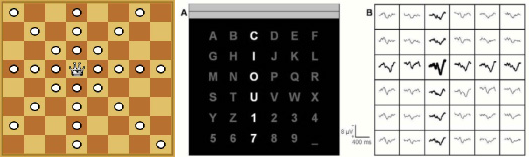
\includegraphics[scale=0.7]{images/QueenControlExample.png}
\caption{Die Bewegungsmöglichkeiten einer Dame deren Zielfeld mit einem P300-Speller ausgewählt werden könnte}
\label{ChessQueen}
\end{center}
\end{figure}

Dies funktioniert allerdings nicht für jede Schachfigur.
Denn eine Dame, ein Läufer und ein Turm können sich nicht nur in verschiedene Richtungen bewegen, sondern auch unterschiedlich weit.
Für diese Steuerung wird eine dem P300-Speller nahe kommende Methode wie in Abbildung\footnote[2]{Bild-Quelle: \cite[S.5]{BCIChess}} \ref{ChessQueen} vorgeschlagen, so dass das Zielfeld auf Basis einer 8x8-Matrix genau ausgewählt werden kann.








\pagebreak
\subsection{Design und Implementierung eines BCI-Schachs}
\label{chessDesignAndImplemention}
Der Artikel \cite{toersche2007designing} befasst sich ebenfalls mit dem Design und der Implementierung einer BCI-Steuerung für Schach.
Dafür werden zunächst die Rahmenbedingungen festgelegt, sodass ein quelloffenes Schach-Spiel und die \acs{BCI2000}-Plattform für die BCI-Steuerung verwendet werden soll.
Die Steuerung soll über einen P300-Speller erfolgen.
In diesem Zusammenhang wird sich mit der Art der Stimuli auseinandergesetzt, ob diese durch Zeilen und Spalten oder einzelne Zellen des Schachbretts dargestellt werden.
Ein P300-Speller der Zellen hervorhebt, kann das Problem haben, dass nicht genügend Zellen zur Verfügung stehen, sodass leere Zellen zur Auswahl hinzugefügt werden müssen.
Dieses Problem tritt beim Zeilen-/Spalten-Speller nicht auf, weshalb ihm der Vorzug zu gewähren ist.
Insbesondere weil die Genauigkeit weiter erhöht werden kann, 
indem nicht erreichbare Zeilen in einigen Spielabschnitten als Ergebnis ausgeschlossen werden können.\\
Ein wichtiger Aspekt auf den das Design eingeht, ist die individuell benötigte Zeit zum Nachdenken.
Da jedem Zug eine gewisse Zeit zum Denken vorausgeht, werden einige Möglichkeiten betrachtet, um dieses Problem zu lösen.
Würde pauschal eine gewisse Zeit zur Verfügung gestellt werden, kann diese in der einen Runde zu viel und in der anderen zu wenig sein.
Ein Lösungsvorschlag dieses Problems ist die Verwendung eines weiteren BCIs, das bei einer imaginären Handbewegung den Zug beginnt, jedoch wird dadurch die Komplexität erhöht.
Alternativ und damit weniger komplex wird diese Option in den Speller integriert, sodass die Auswahl eines unbesetzten Feldes die Denkzeit erhöht.
Für eine eventuelle Implementierung mit einem Zellen-Speller würde einfach eine Zelle außerhalb des Schachbretts dargestellt, deren Auswahl ebenfalls die Denkzeit erhöht.\\
Im weiteren Verlauf wird das Design der Implementierung vervollständigt, sodass die Kommunikation zwischen zwei Spielern über einen Server mittels IRC durchgeführt wird.
Die BCI2000-Plattform kommuniziert über eine Schnittstelle für externe Anwendungen mit einem BCI-Schach-Logik-Modul (BSLM), 
das alle Komponenten miteinander verknüpft, sodass die Signale des BCI vom BCI2000 empfangen und verarbeitet werden.
Die weitere Verarbeitung und Darstellung der Stimuli erfolgt durch das BSLM und das Schachspiel.\\
Abschließend befasst sich die Studie mit einer Analyse der Genauigkeit und der benötigten Zeit pro Zug.
Zu diesem Zeitpunkt ist die Implementierung des Schachspiels jedoch noch nicht abgeschlossen, weshalb die Genauigkeit und die benötigte Zeit nur theoretisch, anhand bestehender Daten anderer Quellen, errechnet wird.\\








\pagebreak
\subsection{Manuelle BCI-Steuerung eines Rollstuhls}
\vspace{0.3cm}

Die Steuerung eines Rollstuhls per \acs{BCI} ist eine erstrebenswerte Anwendung für Patienten mit motorischen Störungen.
\ac{LIS}-Patienten würden auf diese Weise ein gewisses Maß an Eigenständigkeit zurückerlangen und ihre Hilfsbedürftigkeit verringern.
Mit diesem Thema befassen sich deshalb zwei wissenschaftliche Studien (Studie 1 \cite{wheelchairBCI2}, Studie 2 \cite{wheelchairBCI3}), die in den nächsten Seiten genauer betrachtet werden.\\



Beide Studien verwendeten in ihrer Arbeit ein kombiniertes System bestehend aus BCI-Gerät, 
das anhand von mentalen Aufgaben (motorisch und kognitiv) gesteuert wurde und einem intelligentem Rollstuhl, der mit Hilfe eines Lasers die Umgebung abtastete.
Ein Hindernis links vom Rollstuhl bewirkte eine Einschränkung der Bewegungsmöglichkeiten, so dass der Befehl "`Turn Left"' eine Wahrscheinlichkeit von 0\% erhielt.
In den Experimenten beider Studien assoziierte jede Testperson einen Steuerbefehl ("`Turn Left"', "`Forward"' und "`Turn Right"') mit einer mentalen Aufgabe.
Das BCI wertete 16 EEG-Muster pro Sekunde aus und lieferte alle 0,5 Sekunden einen Befehl für den Rollstuhl.
Im der ersten Studie bekamen zwei Testpersonen die Aufgabe in zehn Versuchen 
und in fünf Sitzungen einen vordefinierten Weg in einer virtuellen Umgebung (siehe Abbildung\footnote[1]{Bild-Quelle: \cite[S.2161]{wheelchairBCI2}} \ref{TestEnvWheelchair}) zurückzulegen.\\

\begin{figure}[h!]
\begin{center}
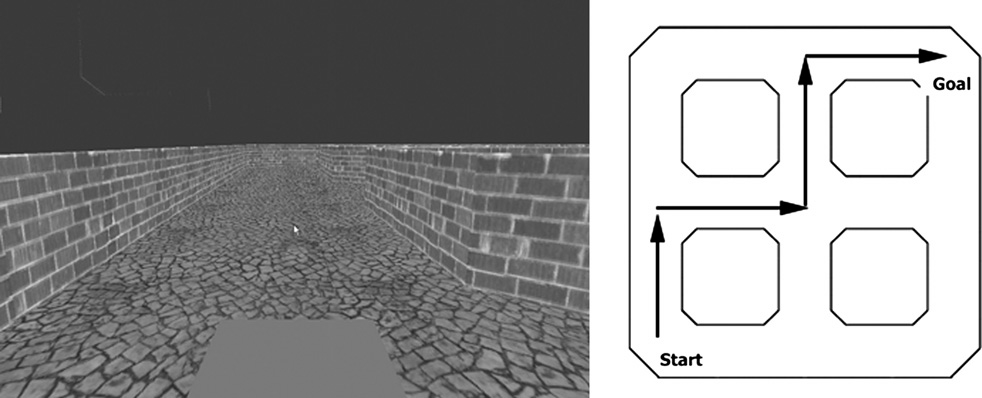
\includegraphics[scale=0.45]{images/TestEnvWheelchair.png}
\caption{Die virtuelle Rollstuhlumgebung und der zu absolvierende Weg.}
\label{TestEnvWheelchair}
\end{center}
\end{figure}

Die erreichten Ziele variierten von 40-100\% und von 10-80\% bei den beiden Testpersonen, wobei die niedrigen Werte am Anfang (40\%, 10\%) mit einem Lernprozess begründet werden. 
Im Vergleich dazu erreichten nur 1\% von 100 zufallsgesteuerten Versuchen innerhalb der Versuchsdauer das Ziel. \\

Darauf aufbauend wurde in der zweiten Studie ein ähnliches Experiment in der realen Welt durchgeführt.
Zusätzlich zu den bisherigen EEG-Daten wurden \ac{EMG}- und \ac{EOG}-Daten erfasst um auszuschließen, 
dass Augenbewegungen oder Muskelaktivität im EEG-Signal fälschlicherweise als Kontrollsignale gewertet werden.\\

In diesem Experiment bestand die Aufgabe darin, auf einem Weg drei Ziele nacheinander zu passieren.
Gemessen wurde dabei wie nah jede Testperson den Zielen bei jedem Versuch kam.
Dem wurde wieder ein Zufallsgesteuertes BCI gegenübergestellt. 
In Abbildung\footnote[1]{Bild-Quelle: \cite[S.8]{wheelchairBCI3}} \ref{WheelchairResults} ist zu sehen, wie weit die einzelnen Testsubjekte bzw. das zufallsgesteuerte BCI vom Ziel entfernt waren.\\

\begin{figure}[h!]
\begin{center}
\includegraphics[scale=0.85]{images/WheelchairResults2.png}
\caption{Testergebnisse des Experiments aus Studie 2. Die zurückgelegte Dis\-tanz ist auf der X-Achse und die prozentual erreichten Ziele auf der Y-Achse abgebildet.}
\label{WheelchairResults}
\end{center}
\end{figure}


Die Ergebnisse zeigten wie schon in der ersten Studie, dass die Personen in der Lage waren einen Rollstuhl in Echtzeit zu kontrollieren 
und damit eine Aufgabe, die schnelle und genaue Entscheidungen abverlangt, zu bewältigen. 
Die Ergebnisse des ersten Experiments in der virtuellen Umgebung schnitten dabei jedoch besser ab als die in der realen Welt, obwohl beide noch weit vom Optimum entfernt sind.











\pagebreak
\subsection{P300-Steuerung eines Rollstuhls mit automatischer Navigation}
\vspace{0.3cm}

Für die Steuerung eines Rollstuhls betrachtet die Studie \textit{"`Synchronous EEG Brain-Actuated Wheelchair with Automated Navigation"'} \cite{WheelchairBCI1} einen anderen Ansatz.
In diesem wird lediglich die Auswahl des Ziels vom Rollstuhlfahrer übernommen, so dass nach Eingabe ein automatisches Navigationssystem den Rollstuhl an sein Ziel steuert.
Für diese Anwendung wurden in einem herkömmlichen elektrischen Rollstuhl zwei Computer verbaut, die für die Motorsteuerung und für die Berechnung der Navigation zuständig waren.
Der Fahrer des Rollstuhls hatte zusätzlich einen Notebook vor sich, über den die visuelle Stimuli-Präsenation durchgeführt wurde. 
Darüber hinaus war der Rollstuhl auch mit einem Laser ausgestattet, sodass Hindernisse in der Navigation und Zielauswahl berücksichtigt werden konnten.
Für die Zielauswahl wurde eine grafische Benutzeroberfläche verwendet, die eine vereinfachte virtuelle Ansicht der Benutzerwahrnehmung darstellte.
Auf der Benutzeroberfläche wurde unter Verwendung des P300-Paradigmas eine Matrix bzw. ein Gitter, wie in Abbildung\footnote[1]{Bild-Quelle: \cite[S.2]{WheelchairBCI1}} \ref{WheelchairGUI} zu sehen, mit vier Zeilen und fünf Spalten dargestellt. 
Die ersten drei Zeilen entsprachen den Zielen und staffelten sich in 8m, 4m und 2m Abständen.
Die fünf Spalten entsprachen jeweils einem Winkel von -60°, -30°, 0°, 30° und 60°.\\

\begin{figure}[h!]
\begin{center}
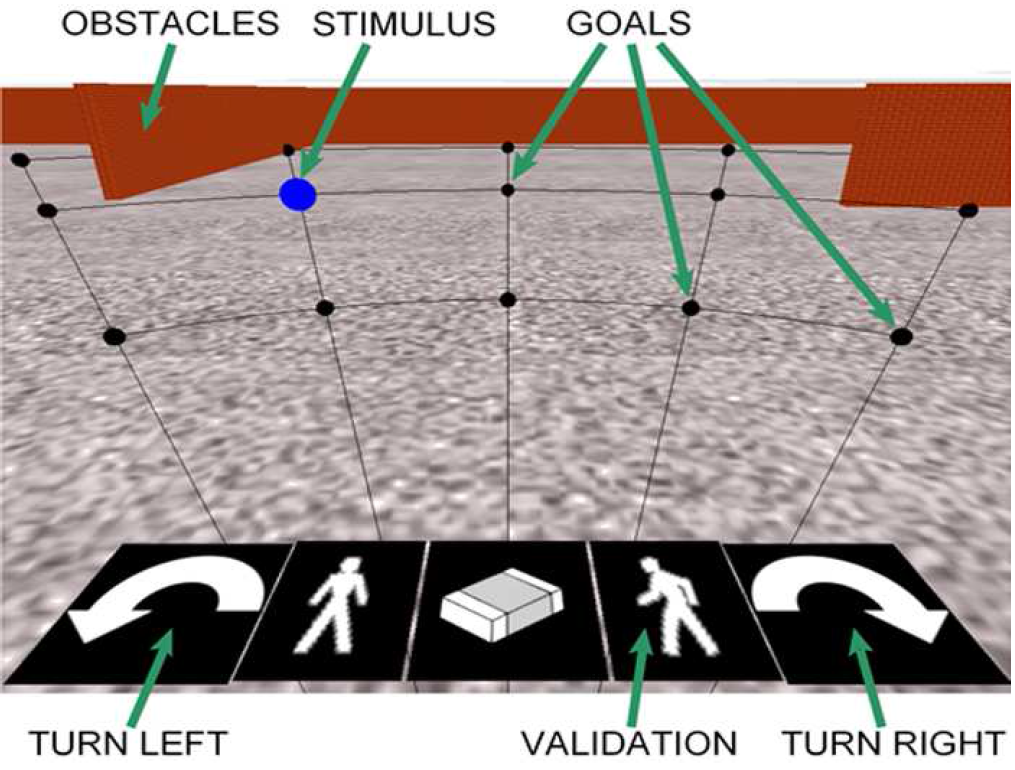
\includegraphics[scale=0.32]{images/WheelchairGUI.png}
\caption{Die grafische Benutzeroberfläche für die Zielauswahl des Rollstuhls.}
\label{WheelchairGUI}
\end{center}
\end{figure}

\pagebreak
Jede Zielauswahl erfolgte in zwei Schritten. Zunächst wurden die Stimuli-Sequenzen abgespielt, sodass ein Zielpunkt ausgewählt werden konnte.
Anschließend musste dieser entweder bestätigt werden, indem das Validierungssymbol ausgewählt wurde 
oder es konnte Schritt eins wiederholt und ein neuer Zielpunkt ausgewählt werden.
Bei erfolgreicher Zieleingabe übernahm das Navigationssystem die Kontrolle, während die BCI-Steuerung in einem Wartezustand verblieb, bis das Ziel erreicht wurde.
Um an das endgültige Ziel zu gelangen waren mitunter mehrere Zwischenziele nötig, sodass die Kontrolle immer zwischen BCI-Steuerung und Navigationsystem wechselte.\\

Das System wurde in einem Experiment mit fünf gesunden männlichen Testpersonen durchgeführt und wurde in drei Phasen unterteilt, die ersten beiden dienten der Unterweisung und dem Training der Testpersonen. 
In der dritten Phase mussten jeweils zwei vordefinierte Routen absolviert werden. 
Dies wurde von allen Testpersonen erfolgreich abgeschlossen.
Die erzielte durchschnittliche Genauigkeit der BCI-Steuerung entsprach während dieser Phase 94\% und zeigt somit eine gute Anwendbarkeit des Systems.\\










\pagebreak
\subsection{Steuerung eines Pinball-Spielautomaten}
\vspace{0.3cm}

Die Studie \textit{"`Playing Pinball with non-invasive BCI"'} \cite{BCIPinball} befasst sich mit der Steuerung eines Pinball-Spielautomaten in Echtzeit.
Für dieses Experiment wurde der Automat präpariert, sodass die Spielbälle ausschließlich an den beiden Kontroll-Paddeln vorbei konnten 
und das Gefälle des Automaten wurde etwas verringert, um das Spiel zu verlangsamen.
Die Steuerung erfolgte unter Verwendung von sensomotorischen Rhythmen. Die Vorstellung einer linken bzw. rechten Handbewegung steuerte die jeweiligen Kontroll-Paddel.
Für die Tests wurden bereits erfahrene BCI-Testpersonen verwendet. Allerdings erreichten nicht alle eine verlässliche Kontrolle über das Spiel, sodass diese von der Bewertung ausgeschlossen wurden.
Alle 0,5 Sekunden wurden die EEG-Daten ausgewertet und in einen Befehl übersetzt. Die Ergebnisse wurden aufgezeichnet und den Ergebnissen einer Pseudo-Zufallssteuerung gegenübergestellt.
Die Qualität der einzelnen Bälle, 
sowie deren Dauer und die Gesamtpunktzahl der Testpersonen war deutlich besser als die der Pseudo-Zufalls-Kontrolle (siehe Abbildung\footnote[1]{Bild-Quelle: \cite[S.7]{BCIPinball}} \ref{PinballBCI}).\\

\begin{figure}[h!]
\begin{center}
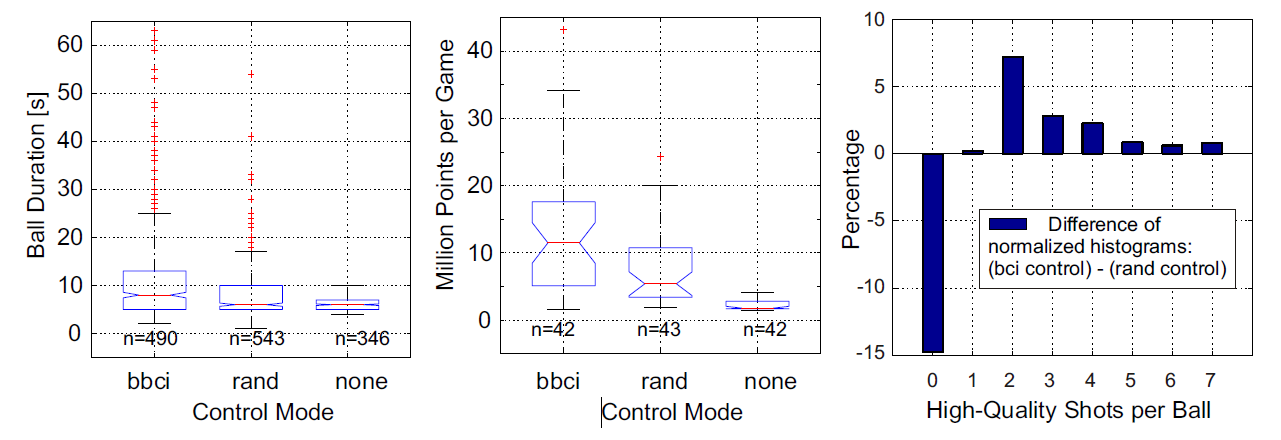
\includegraphics[scale=0.45]{images/PinballBCI.png}
\caption{Die durchschnittlichen Ergebnisse der vier bewerteten Testsubjekte im Vergleich zu den Ergebnissen der Pseudo-Zufalls-Kontrolle, sowie den Ergebnissen, die ohne jede Kontrolleinwirkung erzielt wurden.}
\label{PinballBCI}
\end{center}
\end{figure}

Es zeigt sich damit, dass die Kontrolle eines stark modifizierten Pinball-Spielautomaten in Echtzeit durch ein Brain Computer Interface möglich ist. \\











\pagebreak
\subsection{Stimuli-Präsentation nicht-statischer Objekte}
\vspace{0.3cm}
Das am häufigsten verwendete \acs{BCI} basiert auf dem P300 Paradigma. In den meisten Fällen wird bei den verwendeten BCIs die Stimulation visuell erzeugt.
In äquidistanten Zeitabständen werden Objekte gleichverteilt und in zufälliger Reihenfolge auf dem Bildschirm hervorgehoben.
Dies funktioniert mit vielen Geräten relativ gut, sofern diese über statische Bedienelemente verfügen. 
Bei interaktiven Szenerien stößt dieser Ablauf allerdings an seine Grenzen,
denn beispielsweise sind in Computerspielen sich bewegende Elemente ein signifikanter Bestandteil.\\

Im Rahmen der Studie 
\textit{"`A P300-based Brain-Computer Interface with Stimuli on Moving Objects: Four-Session Single-Trial and Triple-Trial Tests with a Game-Like Task Design"'} 
\cite[S.5ff]{P300Moving} wurde ein experimentelles Spiel erstellt.


\begin{figure}[h!]
\begin{center}
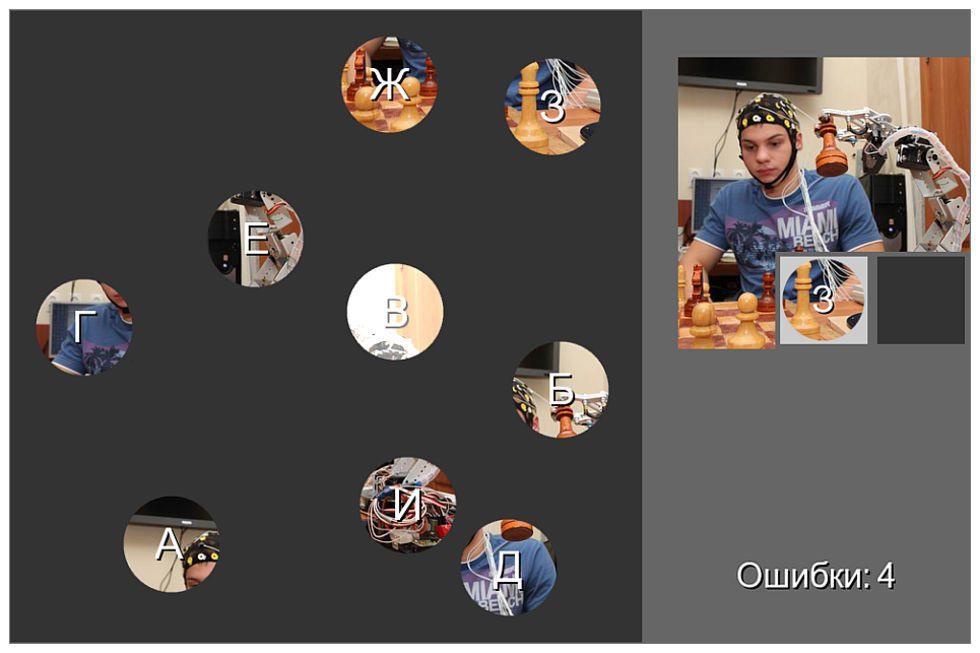
\includegraphics[scale=0.33]{images/MovingStimuliPuzzle.png}
\caption{Die Puzzleteile mit hervorgehobenem Kreis "`B"' und dem bisher zusammengesetzten Puzzle}
\label{MovingStimuliPuzzle}
\end{center}
\end{figure}

Das Ziel des Spiels war, ein Puzzle aus neun Bildfragmenten zusammen zu bauen.
Alle Puzzleteile wurden in gekennzeichneten Kreisen wie in Abbildung\footnote[1]{Bild-Quelle: \cite[S.8]{P300Moving}} \ref{MovingStimuliPuzzle} zu sehen, vor einer schwarzen Fläche angezeigt.
Aus den Kennzeichnungen ergab sich eine alphabetische Reihenfolge, woran sich die Spieler orientieren mussten.
Sobald das Spiel gestartet wurde, bewegten sich die Kreise in zunächst zufällige Richtungen, 
welche im weiteren Verlauf von Kollisionen mit anderen Kreisen oder dem Außenrand beeinflusst wurden.
Die Kreise wurden während sie sich bewegten in zufälliger Reihenfolge hervorgehoben.\pagebreak

Die Aufgabe jedes Spielers war es den Kreis der aktuellen Kennzeichnung zu fokussieren, 
diesen zu verfolgen und sich darauf zu konzentrieren, ob oder wie oft der Kreis aufblitzte.\\
Die Teilnehmer dieses Experiments wurden darüberhinaus in zwei Gruppen aufgeteilt.
Einer Gruppe "`Single-Trial"' wurden pro Durchlauf alle Kreise nur jeweils ein mal hervorgehoben, der anderen "`Triple-Trial"' hingegen jeweils drei mal.
Bei einer falschen Auswahl wurde dem Spieler ein Fehlerpunkt hinzuaddiert. Erreichte ein Spieler zehn Fehlerpunkte, so hatte er das Spiel verloren.
Gewonnen wurde das Spiel, sobald das Puzzle vollständig war.\\

Die Durchführung dieser Tests zeigte auf, dass die Genauigkeit der Ergebnisse beim "`Single-Trial"' geringer war als bei der "`Triple-Trial"'-Gruppe, 
im Umkehrschluss war jedoch das Interesse am Spiel bei der "`Single-Trial"'-Gruppe größer, da ein höherer Spielfluss stattfand.
Das Experiment zeigte, dass das P300 Paradigma sich permanent bewegende Objekte registrieren kann \cite[S12]{P300Moving} und diese Art der Stimuli-Präsentation reale Anwendung finden kann. 
Mit höherem Spielfluss bzw. höherer Geschwindigkeit muss allerdings ein Verlust an Genauigkeit in Kauf genommen werden.\\











\pagebreak
\subsection{Ein auf P300 basierendes haptisches \acs{BCI}}
\vspace{0.3cm}
% Mit Hilfe des \acs{P300 ERP} kann einem Menschen mit dem sogenannten \ac{LIS} eine Möglichkeit gegeben werden, mit seiner Umwelt zu kommunizieren.
% Patienten mit \acs{LIS} sind in ihrem Körper gefangen, sie verfügen nicht über die Möglichkeit der Selbstdarstellung, obwohl sie bei vollem Bewusstsein sind.
% Viele aktuelle \acs{BCI} Anwendungen ermöglichen Kommunikation, indem sie \acs{P300 ERP}'s evozieren.

Bei einer Person mit einem eingeschränkten Bewusstsein bzw. ohne ein mindestmaß an visueller Wahrnehmung, ist eine visuelle Stimulation und eine darauf basierende Kommunikation nicht möglich.
Unabhängig davon verfügen viele betroffene Menschen weiterhin über ihren Tastsinn.\\
In der Studie \textit{"`A Tactile P300-Based BCI"'} \cite[Art. 98]{P300Tactile} wurde ein auf dem Tastsinn und dem \acs{P300 ERP} basierendes \acs{BCI} präsentiert.
Dieses ermöglicht einer Person die Kommunikation mittels haptischer Stimulation.
Hierfür wurden drei Szenarien getestet, in denen die Stimuli repräsentiert durch kurze Vibrationen einen \acs{P300 ERP} evozierten.\\

\begin{itemize}

\item[\textbf{Szenario 1: }] Den Testpersonen wurden jeweils zwei Stimulatoren an die Handgelenke angelegt. 
Einer der Stimulatoren vibrierte in regelmäßigen, der andere in unregelmäßigen Abständen. 
Wenn sich die Testpersonen auf die unregelmäßigen Vibrationen konzentrierten, löste dies zuverlässig ein \acs{P300 ERP} aus.

\item[\textbf{Szenario 2: }] In diesem Szenario wurden drei Stimulatoren verwendet, der dritte befindet sich hierbei auf dem Rücken und vibriert in regelmäßigen Abständen.
Auf diese Weise ist es möglich, mit den beiden Stimulatoren an den Handgelenken, einfache Ja/Nein-Antworten zu erzeugen.

\item[\textbf{Szenario 3: }] Im dritten Szenario wurden die Hände der Probanden mit vier Stimulatoren, jeweils einem pro Finger mit Ausnahme des Daumens versehen.
Jeder dieser Stimulatoren wurde mit gleicher Wahrscheinlichkeit zum vibrieren gebracht.
Die Testpersonen mussten sich in jedem Testlauf in zufälliger Reihenfolge auf einen Finger konzentrieren,
so dass für jeden Finger ein \acs{P300 ERP} erzeugt wurde.\\
\end{itemize}

Die mittlere Genauigkeit aller Probanden der drei Szenarien lag bei 100\%, 80\% und 69,4\%.






\pagebreak
\section{Einordnung in den State of the Art}

Diese Masterarbeit lässt sich im Vergleich zu den meisten behandelten Studien nicht eindeutig einordnen.
Im Bereich der Konzeption einer BCI-Anwendung ist sie vergleichbar mit der Studie "`Brain Chess – Playing Chess using Brain Computer Interface"' von Seite \pageref{chessconcept}, 
allerdings behandelt diese Studie nur die theoretischen Realisierungsmöglichkeiten und kann keine Implementierung vorweisen.\\

Einen Schritt weiter ist die darauf folgende Studie auf Seite \pageref{chessDesignAndImplemention}, diese befasst sich zwar auch weitestgehend mit der Planung eines Schachspiels, 
jedoch wird das Gesamtkonzept tiefergehend betrachtet. 
Hierzu gehört die Verknüpfung der \acs{BCI2000}-Plattform und dem Spiel durch ein BCI-Schach-Logik-Modul als Schnittstelle.
Diese Masterarbeit lässt sich daher im Bereich dieser Studie einordnen, da diese ebenso eine Möglichkeit zur Steuerung eines Spiels plant und realisiert.\\

Alle weiteren Studien befassen sich ebenfalls mit möglichen BCI-Anwendungen, insbesondere mit einigen Anwendungen des \acs{P300 ERP}, 
allerdings sind diese mehr auf die Ergebnisse der jeweiligen Experimente fokussiert und beschreiben weniger die Implementierungsmöglichkeiten für vergleichbare BCI-Erweiterungen.
Die Genauigkeit ist darüberhinaus bei allen Studien ein wichtiger Betrachtungspunkt. 
In Bezug auf diese Arbeit kann daher vorallem eine Balance zwischen Genauigkeit und Spielfluss erforderlich sein, 
da ein zu langsamer Spielfluss möglicherweise die Aufmerksamkeit und damit die Genauigkeit verschlechtern könnte.\\























	
    % 4) Konzeption - Genaue Problembeschreibung (Anforderungsanalyse). Lösungsansatz.
	\chapter{Konzeption}

Innerhalb dieses Kapitels werden verschiedene Teilbereiche dieser Masterarbeit erfasst und für jede Teilaufgabe ein Konzept erstellt.
Inhalt der Konzepte ist unter anderem die Definition der Aufgabe, sowie aller Komponenten, die zur Realisierung benötigt und verwendet werden.\\

An dieser Stelle wird das von der Universität zur Verfügung gestellte Emotiv EPOC als das \acs{BCI} für die späteren Tests der vorliegenden Arbeit definiert. \\


\section{Auswahl der BCI-Software}

Das Forschungsgebiet \acs{BCI} ist in den vergangenen Jahren immer umfangreicher geworden, so existieren mittlerweile eine ganze Reihe von Software Plattformen für die Arbeit mit \acs{BCI}s.
Die ausgewählte Software sollte möglichst alle nachfolgenden Kriterien erfüllen:

\begin{itemize}
\setlength{\itemsep}{0pt}
\footnotesize
{
\item Offener Quellcode
\item Nicht-kommerzielle Verwendung
\item Gute Dokumentation
\item Große und aktive Nutzergemeinschaft
\item Programmiersprache C++, C\# oder Java
\item Gute Software-Architektur für Erweiterungen oder Neuentwicklungen
\item Unterstützung des Emotiv EPOC und möglichst vieler anderer \acs{BCI}'s\\
}
\end{itemize}

Für diese Auswahl werden die \acs{BCI}-Software Plattformen BCI2000, OpenVibe, TOBI und BCI++ kurz vorgestellt, um darauf aufbauend die \acs{BCI}-Software für diese Masterarbeit auszuwählen.
Wichtig bei der Entscheidung ist die vorausgesetzte die Unterstützung des Emotiv EPOC Neuroheadset \cite{Emotiv2014}. \\


\subsubsection{BCI2000}
\acs{BCI2000} \cite{BCI2000Online} ist eine quelloffene Mehrzweckplattform für die Erforschung, Entwicklung und Verwendung von Brain Computer Interfaces. Sie ist in C++ geschrieben und in einer modularen Architektur aufgebaut. 
Sie unterstützt in der aktuellen Version das Betriebssystem Windows, zukünftig soll auch Linux und MacOS hinzugefügt.
Gegenwärtig werden 18 verschiedene Möglichkeiten der EEG-Datenakquirierung und viele Module zur Signalverarbeitung bereitgestellt. 
Darüberhinaus existiert eine umfangreiche Dokumentation für die Benutzung und Entwicklung von \acs{BCI2000}.\\


\subsubsection{BCI++}
BCI++ \cite{BCI++Online} ist ein in C++ entwickeltes Framework zur Erstellung prototypischer \acs{BCI}-Systeme und unterstützt eine Vielzahl an BCI- und Bio-Signal-Paradigmen. 
Der Aufbau des Frameworks ist in zwei Module unterteilt. Dem "`Hardware Interface Module"' (\acs{HIM}) und dem "`Graphical User Interface Module"' bezeichnet als \acs{AEnima}.
Das \acs{HIM} erhält und verarbeitet alle Signale und kommuniziert via TCP/IP mit \acs{AEnima}. 
\acs{AEnima} ermöglicht daraufhin die Realisierung der visuellen Präsentation unter Verwendung der Irrlicht 3D Engine \cite{IrrlichtOnline}. \\


\subsubsection{OpenVibe}
OpenVibe \cite{OpenVibeOnline} ist eine quelloffene in C++ entwickelte BCI-Software Plattform und wird regelmäßig vom \textit{"`French National Institute for Research in Computer Science and Control"'} aktualisiert. 
Sie ist auf das Erstellen, Testen und Benutzen von BCIs spezialisiert.
Zu diesem Zweck ermöglicht sie Nutzern ohne Programmierkenntnisse die Verwendung einer dazugehörigen Grafischen Benutzeroberfläche. 
OpenVibe verfügt über 15 verschiedene Möglichkeiten der EEG-Datenakquirierung (Stand: \today) und unterstützt die Betriebssysteme Windows und Linux.\\


\subsubsection{TOBI}
\ac{TOBI} ist ein europäisches Gemeinschaftsprojekt verschiedener Universitäten und medizinischer Einrichtungen \cite{TOBIOnline}.
Das Ziel ist die Entwicklung praktischer \acs{BCI}-Technologien. 
Es versucht in erster Linie die Interoperabilität zwischen unterschiedlichen \acs{BCI}'s zu erleichtern \cite{BCIPlatforms}.
Deshalb adres\-siert \acs{TOBI}, im Gegensatz zu den bereits vorgestellten BCI-Software Plattformen, insbesondere Entwickler, um die Kompatibilität zwischen anderen \acs{BCI}-Produkten oder -Komponenten zu verbessern.
Darüberhinaus versucht \acs{TOBI} die Standardisierung von BCIs zu erreichen.\\


Die Wahl der BCI-Software Plattform in dieser Arbeit fiel auf BCI2000.
Alle anderen hier vorgestellten Alternativen sind damit in keinster Weise als ungeeignet zu bezeichnen, da die Kriterien ebenfalls von fast allen erfüllt wurden.
Ausschlaggebend für die Entscheidung war daher hauptsächlich die modulare Architektur von BCI2000, 
da die Unterteilung in "`Source"'-, "`Signal-Processing"'- und "`User-Application"'-Modul sehr präzise den Einstiegspunkt dieser Arbeit abgrenzt.
Somit kann ein "`User-Application"'-Modul erstellt werden, während andere für diese Arbeit nicht relevanten Bereiche unangetastet bleiben.
Außerdem verfügt BCI2000 über eine sehr umfangreiche Dokumentation und findet häufig Verwendung in wissenschaftlichen Veröffentlichungen.
BCI2000 konnte zudem gegenüber OpenVibe mehr unterstützte BCIs vorweisen, weshalb dies als ein weiteres Kriterium für BCI2000 gewertet wurde.\\




\pagebreak
\section{Auswahl der Point\&Click Game Engine}
Die Auswahl der Point\&Click Game Engine ist ein sehr wichtiger Aspekt dieser Arbeit. 
Die für die Auswahl wichtigen Kriterien sind:

\begin{itemize}
\setlength{\itemsep}{0pt}
\footnotesize
{
\item Offener Quellcode
\item Nicht-kommerzielle Verwendung
\item Gute Dokumentation
\item Große und aktive Nutzergemeinschaft
\item Möglichkeiten zur Erweiterung der Engine
\item Programmiersprache C++, C\# oder Java\\
}
\end{itemize}

Nachfolgend werden einige untersuchte Point\&Click Game Engines vorgestellt.\\

\subsubsection{ALPACA}
Bei ALPACA \cite{AlpacaOnline} handelt es sich um eine quelloffene und frei verfügbare Point\&Click Game Engine.
Sie ist für die Erstellung von Flash-Anwendungen entwickelt worden. 
Mit ihrer Hilfe sollen Benutzer ohne Programmierkenntnisse im Stande sein eigene Point and Click Spiele zu erstellen.
Der Internetpräsenz ist jedoch zu entnehmen (Stand: \today), dass die Engine zwar weiterhin verwendet werden kann, deren Entwicklung allerdings nicht weiter fortgeführt wird.\\


\subsubsection{Adventure Game Studio}
Das \acf{AGS} ist eine quelloffene Point\&Click Game Engine, die in C++ geschrieben wurde und auf Microsofts .NET Framework basiert.
Sie besteht aus der eigentlichen Engine und einem Editor zur Erstellung der Spiele. 
Sie verfügt über ein Plugin-System für Engine und Editor und ermöglicht somit in Kombination mit Hilfe der umfangreichen Dokumentation, 
eine einfache Funktionserweiterung zur Design- oder Laufzeit des Spiels. 
Die Engine verfügt weiterhin über eine große und aktive Nutzergemeinschaft.\\

\subsubsection{Wintermute Engine}
Die Wintermute Engine ist eine weitere Point\&Click Game Engine, welche ebenfalls in C++ entwickelt wurde.
Ihr Quellcode ist ebenso frei verfügbar und kann somit erweitert werden. 
Der Funktionsumfang ist mit dem des Adventure Game Studios zu vergleichen.
Diese Engine besitzt ebenfalls eine große Dokumentation. \\

\subsubsection{Weitere Point\&Click Engines}
Es existieren eine Reihe weiterer Point\&Click Game Engines, deren Möglichkeiten ziemlich variieren. 
Viele dieser Engines sind jedoch für die Zwecke dieser Arbeit ungeeignet, da ihr Funktionsumfang unzureichend ist.
Am Beispiel der "`Visionaire Studio"' Engine  zeigt sich hingegen eine Engine, die zwar sehr mächtig, jedoch nur kommerziell verfügbar und somit ebenfalls ungeeignet ist.\\\\


Im Rahmen der Konzepterstellung dieser Masterarbeit wurde entschieden die Point\&Click Game Engine \textit{"`Adventure Game Studio"'} zu verwenden.
Die Erweiterbarkeit der Engine durch freie Verfügbarkeit des Quellcodes und des integrierten Plugin-Systems erscheint optimal für das Ziel dieser Arbeit.
Die umfangreiche Dokumentation und die bestehende große und aktive Nutzergemeinschaft, 
die die BCI-Erweiterung und dessen Funktionen aktiv nutzen könnte, 
spielte bei dieser Entscheidung ebenso eine wichtige Rolle.\\



\pagebreak
\section{Auswahl der Kontrollstrategie}
Für die Verwendung von BCIs gibt es verschiedene Strategien, anhand derer die Steuerung erfolgen kann.
In diesem Abschnitt werden einige Strategien vorgestellt und letztlich die Strategie ausgewählt, die den Bedürfnissen der Aufgabe am ehesten gerecht wird.\\



\subsubsection{Sensomotorischer Rhythmus}
Hierbei handelt es sich um Oszillationen im elektrischen Feld, die über dem Sensomotorischen Cortex aufgezeichnet werden.
In den meisten Studien werden für diese Zwecke die $\mu$- (8-12Hz) und $\beta$-Frequenzbänder (18-30Hz) verwendet.
Bei der Betrachtung dieser sensomotorischer Rhythmen \cite[S.227ff]{wolpaw2012braincomputer} (\acs{SMR}) zeigt sich, das sich ihr Verhalten bei realer und imaginärer Bewegung verändert.
Dies zeigt sich anhand einer ereignis\-korrelierten Desynchronisation der Oszillation. 
Die korrespondierenden Signale verschiedener Bereiche wie Hand und Fuß können voneinander unterschieden werden, 
sodass bestimmte Befehle mit der Vorstellung einer Hand- oder Fußbewegung assoziiert werden können.\\



\subsubsection{\ac{SSEP}}
Diese Strategie \cite[S.241ff]{wolpaw2012braincomputer} stellt wiederholende Stimuli dar, um stabile Oszillationen in den EEG-Signalen zu erzeugen.
Je nach Wahl der Frequenz verändert sich die Amplitude der Oszillationen.
Insbesondere deshalb ist es möglich verschiedene Muster anzulegen, deren Frequenz und Amplitude bekannt sind.
Das Signal des Nutzers wird mit den Mustern verglichen, sodass die beste Korrelation dem Ziel-Stimulus entspricht.
Die Stimuli können bei dieser Strategie visuell, akkustisch oder haptisch evoziert werden, allerdings sind jeweils unterschiedliche Gehirnareale betroffen.
Insbesondere ist für die visuelle Darstellung Hardware mit ausreichend hoher Bildwiederholfrequenz erforderlich.\\


\subsubsection{P300 Ereigniskorrelirte Potentiale (\acs{P300 ERP})}
\acs{P300 ERP}'s werden durch seltene Ereignisse ausgelöst die in Konkurrenz zu häufigen Ereignissen stehen und folgen dem Oddball-Paradigma.
Hierbei werden Stimuli in zufälliger Reihenfolge hervorgehoben. 
Der Stimuli der im Fokus eines Nutzers ist, erzeugt ein unterscheidbares \acs{P300 ERP}, sobald es hervorgehoben wird.
Das Objekt, dem das Potential zugeordnet ist, wird ausgewählt.
Mit der Verwendung einer Matrix \cite{FarwellDonchin1988} kann dies erweitert werden, sodass durch die Kombination einer ausgewählten Zeile und Spalte ein Matrix-Element ermittelt werden kann.\\ \\





Die \acs{SMR}-Strategie erscheint wenig geeignet für diese Arbeit, da eine Maus zu bewegen und zu klicken mindestens fünf verschiedene Assoziationen erfordern würde,
da die Unterscheidung zwischen linker und rechter Hand jedoch schon schwer fällt, sind die eindeutigen Ergebnisse begrenzt.
Die Strategie des \acs{SSEP} erscheint ebenfalls wenig sinnvoll. Die Assoziation eines Musters mit einem Befehl ist zwar möglich, 
darüberhinaus sind mögliche Ziele jedoch durch die Anzahl der Muster limitiert.
Die \acs{P300 ERP}-Strategie ist offenbar die sinnvollste Herangehensweise für diese Arbeit, 
da mit einer Matrix und der Auswahl eines bestimmten Matrix-Elements die Simulation eines Mausklicks erfolgen kann.

Somit wird an dieser Stelle das \textit{P300 ereigniskorrelierte Potential} als Kontrollstrategie für die Ausarbeitung des Konzepts festgelegt.\\













\pagebreak
\section{Gesamtkonzept der BCI-Erweiterung}

Auf Basis der ausgewählten BCI-Software Plattform und der Point\&Click Game Engine wird in den nächsten Seiten ein Grundkonzept erarbeitet.
Einführend wird eine Übersicht (Abbildung \ref{Overview}) aller involvierten Komponenten der BCI-Erweiterung gegeben, anhand derer die Abläufe und Zustände dargestellt werden.
Zu diesem Zweck wird jede der zu entwickelnden Komponenten einzeln ausgearbeitet, um die erforderlichen Funktionen, Parameter und Abhängigkeiten zu definieren.\\

\begin{figure}[h!]
\begin{center}
\begin{tikzpicture}[scale=1.08,
bci/.style={rectangle,draw=black!50,fill=blue!20},
bci2/.style={rectangle,draw=red!70,fill=blue!20},
game/.style={rectangle,draw=black!50,fill=green!20},
game2/.style={rectangle,draw=red!70,fill=green!20},
rechteck/.style={rectangle,draw=black!50,minimum height=17mm,minimum width=22mm},
display/.style={rectangle,draw=black!50,fill=yellow!20,minimum height=20mm,minimum width=25mm},
empty/.style={rectangle,draw=black!0,fill=black!0}]


% BCI2000
\def\X{5}
\node (bci2000) at (\X,0.75) {\textbf{BCI2000}};
\node[bci] (operator) at (\X,0) {Operator};
\node[bci2] (application) at (\X,-0.75) {Application};
\node[bci] (signal) at (\X,-1.5) {Signal Processing};
\node[bci] (source) at (\X,-2.25) {Source};
\draw (3,0.5) -- (7,0.5) -- (7,-2.75) -- (3,-2.75) -- (3,0.5);

\node at (0,0.02) {TCP/IP-Kommunikation};

% Point and Click Game
\def\X2{-5}
\node (game) at (\X2,0.75) {\textbf{Point\&Click-Spiel}};
\node[game2] (plugin) at (\X2,0) {AGS Engine Plugin};
\node[game] (game) at (\X2,-1) {AGS Game};
\draw (-2.9,0.5) -- (-7.1,0.5) -- (-7.1,-1.5) -- (-2.9,-1.5) -- (-2.9,0.5);

% Monitor
\node[display] (display) at (0,-1.75) {Monitor};
\node[rechteck] (display) at (0,-1.75) {Monitor};

% Subject
\node[empty] (subjectTop) at (0,-4) {};
\node[empty] (subjectRight) at (0.631,-4.45) {};
\draw[fill=pink!30] (0,-4.7) ellipse (0.75 and 0.8);
\node (userbci) at (0,-5.7) {\textbf{Benutzer mit BCI}};
\node at (3.75,-4.0) {EEG-Datenerfassung};

% Arrows
\draw [<->] (application) -- (plugin);
\draw [<->] (game) -- (plugin);
\draw [->] (game) -- (display);
\draw [->] (application) -- (display);
\draw [->] (display) -- (subjectTop);
\draw [->] (subjectRight) -- (source);

\end{tikzpicture}
\caption{Eine einfache Übersicht der einzelnen Bestandteile und deren Zusammenhänge. Die zu entwickelnden Kernkomponenten der BCI-Erweiterung sind mit einer roten Umrandung versehen.}
\label{Overview}
\end{center}
\end{figure}




\subsubsection{Die zu realisierenden Komponenten dieser Arbeit}
\begin{itemize}
\item Das Anwendungsmodul für BCI2000
\item Das AGS Engine Plugin, mit dessen Hilfe das Anwendungsmodul des \acs{BCI2000} mit dem Spiel kommunizieren und die Parameter austauschen kann.
\item Ein Point\&Click Spiel, welches die \acs{BCI}-Steuerung des AGS Engine Plugins verwendet und demonstriert.
\end{itemize}





\pagebreak
\section{Das BCI2000 Anwendungsmodul}

Dieses Kapitel behandelt die Definition, Auswahl und Planung des BCI2000 Anwendungsmoduls.

\subsection{Szenarien}
\vspace{0.3cm}
Im Zuge der Konzeption existierten zwei zu betrachtende Möglichkeiten, wie das Anwendungsmodul realisiert werden könnte.

\begin{itemize}
\setlength{\itemsep}{0pt}
\footnotesize
{
\item[1.] Implementierung der P300-Speller Funktionalitäten innerhalb des AGS Engine Plugins als sogenannte "`External Application"' des \acs{BCI2000}
\item[2.] Implementierung eines Anwendungsmoduls für die Verarbeitung von Speller-Matrix-Anfragen des \acs{AGS} Engine Plugins, basierend auf dem bestehenden P300 Speller des \acs{BCI2000}\\
}
\end{itemize}

\subsubsection{Szenario 1}
Das erste Szenario würde die Engine-Erweiterung und das BCI2000 Anwendungsmodul kombinieren. 
Dies würde mit sich bringen, dass sehr nah an der Engine gearbeitet wird und dortige Werkzeuge für die Visualisierung verwendet werden könnten.
Allerdings ist an dieser Stelle nicht bekannt, welche Möglichkeiten sich daraus ergeben und in wie weit diese limitiert sind, 
insbesondere da die Engine auf die Verwendung der Grafikbibliothek "`Allegro"' in der Version 4 begrenzt ist.
Bei der Untersuchung der \acs{BCI2000}-Plattform stellte sich jedoch heraus, 
dass die Architektur des bestehenden P300-Spellers und die Verknüpfung der Stimuli-Assoziationen zwischen P300-Speller 
und "`Source"'-Modul sehr komplex und besonders zeitkritische Faktoren sind.

\subsubsection{Szenario 2}
Die zweite Möglichkeit wäre die Entwicklung eines Anwendungsmoduls auf Basis des bestehenden P300-Spellers.
Auf diese Weise wären \acs{AGS} Engine Plugin und Anwendungsmodul zwei getrennte Komponenten, welche lediglich via TCP/IP miteinander kommunizieren.
Der daraus resultierende "`AGS-P300-Speller"' würde vor jeder Anfrage des Spiels die entsprechenden Parameter zugesendet bekommen. 
Die Größe, Position und der Typ der Speller-Matrix, sowie das aktuelle Bild des Spiel-Auschnitts würden alles abdecken, sodass der Speller darauf arbeiten könnte.
Hierbei würde im Hintergrund das Bild dargestellt werden und die Speller-Matrix würde auf dieses Bild überlagert werden, um die Eingaben zu ermitteln.
Diese Variante würde es theoretisch ermöglichen, dass zusätzliche Erweiterungen für andere Spiele Engines entwickelt werden könnten, welche auf die gleiche Weise mit dem Speller kommunizieren könnten.\\\\

\subsubsection{Auswahl des Szenarios}
Szenario 2 ist nach Abschluss der Recherche im Rahmen dieser Masterarbeit am sinnvollsten, da diese Variante basierend auf dem bestehenden P300-Speller auf ein funktionierendes Konzept aufbaut.
Denn durch eine potentielle Neuentwicklung des P300-Spellers besteht die große Gefahr, dass der "`AGS-P300-Speller"' nicht korrekt funktioniert.

Insbesondere müssen die Stimuli des Spellers mit den entsprechenden Signalen des "`Source"'-Moduls verknüpft werden.
Die Visualisierung der Stimuli und deren Assoziation spielt sich jedoch im Millisekunden-Bereich ab und ist somit generell zeitkritisch.\\

Eine Neuentwicklung und ein damit verbundener Mehraufwand zur Fehlerbehebung könnte möglicherweise den zeitlichen Rahmen dieser Masterarbeit übersteigen 
und ist demzufolge ein nicht kalkulierbares Risiko, das die Auswahl des 2. Szenarios begründet.\\







\pagebreak
\subsection{Konzept}

Das \acs{BCI2000} Anwendungsmodul kann für sich selbst in einem Aktivitätsdiagramm (siehe Abbildung \ref{aktivitaetsdiagrammbci2000}) dargestellt werden. 
Zunächst wird es zusammen mit der \acs{BCI2000}-Plattform gestartet und geht in eine Warteschleife über. 
In dieser Schleife wartet es auf eine Anfrage des AGS Engine Plugins oder einen Beenden-Befehl.
Sobald eine Anfrage erhalten wurde, werden die darin enthaltenen Parameter ausgewertet.
Aus den Parametern wird die Speller-Matrix aufgebaut und der aktuelle Bildausschnitt in den Hintergrund gelegt, so dass anschließend die Stimuli-Sequenzen vor diesem Hintergrund visualisiert werden.
Nach Abschluss dieser Prozedur wird das Ergebnis zurück an das AGS Engine Plugin gesendet und der Speller betritt bis zur nächsten Anfrage wieder die Wartschleife. \\\\




\begin{figure}[h!]
\begin{center}
\begin{tikzpicture}[scale=1.08,
rect0/.style={line width=2pt,rectangle,draw=black!100,fill=red!10,minimum width=33mm,text width=30mm,minimum height=15mm,align=center, rounded corners},
rect1/.style={rectangle,draw=black!70,fill=blue!10,minimum width=33mm,text width=30mm,minimum height=15mm,align=center, rounded corners},
rect2/.style={rectangle,draw=black!70,fill=green!10,minimum width=33mm,text width=30mm,minimum height=15mm,align=center, rounded corners},
rect3/.style={rectangle,draw=black!70,fill=yellow!10,minimum width=33mm,text width=30mm,minimum height=15mm,align=center, rounded corners},
circle1/.style={circle,draw=black!100,fill=black!100,minimum width=5mm,minimum height=5mm,align=center},
circle2/.style={circle,draw=black!100,fill=black!0,minimum width=7mm,minimum height=7mm,align=center},
]

% BCI2000 Aktivitätsdiagramm
\node at (20mm, 0) {AGS-P300-Speller};

\node at (-40mm, -0.45) {Start/Stop};
\node[circle2] (start) at (-40mm, -1) {};
\node[circle1] at (-40mm, -1) {};
\node[rect3] (params) at (-40mm, -3) {Auf Para\-meter warten};
\node[rect1] (setup) at (0mm, -3) {Speller-Matrix aufbauen};
\node[rect2] (sequence) at (40mm, -3) {Stimulus Sequenzen durchführen};
\node[rect1] (result) at (80mm, -3) {Ergebnis zurück senden};

\path[->] 	(params) 	edge 					node {} (setup)
			(setup) 	edge 					node {} (sequence)
			(sequence) 	edge 					node {} (result)
			(result) 	edge 		 [bend left]node {} (params)
			(start) 	edge 		 [bend left]node {} (params)
			(params) 	edge 		 [bend left]node {} (start)
			(params)	edge 		[loop below]node {} (params);
			
\end{tikzpicture}
\caption{Das Aktivitätsdiagramm des AGS-P300-Spellers.}
\label{aktivitaetsdiagrammbci2000}
\end{center}
\end{figure}










\pagebreak
\section{Das \acs{AGS} Engine Plugin}
Da für das Anwendungsmodul Szenario 2 ausgewählt wurde, wird das AGS Engine Plugin lediglich die Verbindung herstellen 
und die Kommunikation zwischen dem Spiel und dem \acs{AGS}-P300-Speller übernehmen.
Dafür muss die Erweiterung Methoden bereitstellen, so dass Eingabe-Anfragen an den Speller gesendet werden können. 
Die Speller-Matrix Parameter sind zugleich auch die benötigten Parameter der entsprechenden Methode.
Lediglich den aktuellen Bildausschnitt holt sich das Plugin direkt von der Engine. 
Das Flussdiagramm des Spiels und des Plugins sind in Abbildung \ref{diagrammplugin} zu sehen. \\ \\


\begin{figure}[h!]
\begin{center}
\begin{tikzpicture}[scale=1.08,
rect0/.style={line width=2pt,rectangle,draw=black!100,fill=red!10,minimum width=33mm,text width=30mm,minimum height=15mm,align=center, rounded corners},
rect2/.style={rectangle,draw=black!70,fill=green!10,minimum width=33mm,text width=30mm,minimum height=15mm,align=center},
rect3/.style={rectangle,draw=black!70,fill=black!10,minimum width=33mm,text width=30mm,minimum height=15mm,align=center, rounded corners},
raute/.style={rectangle,rotate=45,draw=black!100,fill=black!0,minimum width=20mm,minimum height=20mm, align=center}]

% AGS Engine Plugin Aktivitätsdiagramm

\draw (-6.5,0) -- (2.5,0) -- (2.5,-9) -- (-6.5,-9) -- (-6.5,0);
\node (a) at (-4, -0.5) {Point\&Click Spiel};
\node (b) at (0, -0.5) {AGS Engine Plugin};


%\node[rect3] (game) at (-4, -2) {};
\node[rect3] (game) at (-4, -2) {Spiel};

\node[raute] (check) at (-4, -5) {};
\node at (-4, -5) {Eingabe?};
\node at (-4.3, -6.7) {Ja};
\node at (-5.1, -3.5) {Nein};
\node[rect2] (control) at (-4, -8) {Anfrage an Plugin senden};

\node[rect2] (result) at (0, -8) {Warte auf Ergebnis};
\node[raute] (check2) at (0, -5) {};
\node at (-0, -5) {Ergebnis?};
\node at (1.15, -6.55) {Nein};
\node at (-0.9, -2.6) {Ja};

\draw [<->] (a) -- (b);

\path[->]	 (game)		edge 	     [bend left]node {} (check)
			 (check)	edge 	     [bend left]node {} (game)
			 (check)	edge 					node {} (control)
			 (control)	edge 					node {} (result)
			 (result)	edge 		[bend left] node {} (check2)		
			 (check2)	edge 		[bend left] node {} (result)			
			 (check2)	edge 		[bend right] node {} (game);
			
\end{tikzpicture}
\caption{Das Flussdiagramm zwischen Spiel und AGS-P300-Speller Plugin}
\label{diagrammplugin}
\end{center}
\end{figure}




\pagebreak
\section{Point\&Click Test-Spiel}

Im Anschluss an die Implementierung der BCI-Erweiterung wird in diesem Abschnitt ein einfaches Test-Spiel konzipiert.
Dieses Spiel soll im späteren Verlauf für Tests verwendet werden, so dass Ergebnisse gesammelt und ausgewertet werden können.\\

Das Test-Spiel soll ein kurzes und einfaches Szenario darstellen, so dass die späteren Testpersonen lediglich einige Eingaben durchführen müssen um eine Aufgabe zu erfüllen.
Das Szenario wird gemäß des Titels dieser Masterarbeit an "`The Secret of Monkey Island"' angelehnt sein und sich daher optisch in diese Richtung orientieren.
Die Aufgabe wird es sein einen fiktiven Charakter über einen Strand laufen zu lassen und mit anderen Charakteren zu reden oder Gegenstände aufzuheben, 
um diese an einen Zielort zu bringen. 
Die Eingabe würde über einen P300-Speller erfolgen.\\

In Abbildung \ref{gameconcept} ist eine Skizze zu sehen, wie die Spielszene aussehen könnte.
Ein Befehl an die Spielfigur würde dann so ablaufen, dass zunächst mit dem Speller ein Befehl in der unteren GUI-Leiste ausgewählt und anschließend ein Ziel für diesen Befehl ermittelt wird.
Je nach ausgewählten Befehl kann sich die Position der Speller-Matrix entsprechend an die Position der möglichen Ziele anpassen.
Da die Speller-Matrix eine gewisse Mindestgröße benötigt, kann es hier durchaus nötig sein, dass eine Schaltfläche für einen Befehl durch mehrere Zeilen und Spalten abgedeckt werden muss.


\begin{figure}[h!]
\begin{center}
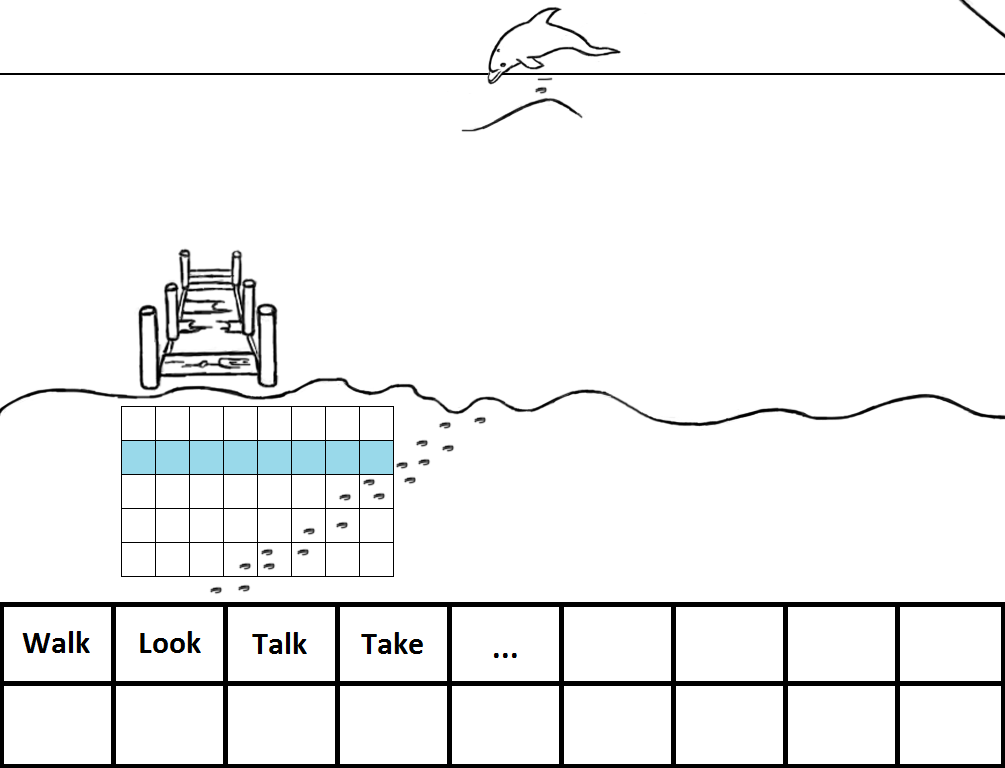
\includegraphics[scale=0.3]{images/szene1konzept.png}
\caption{Skizze einer Szene mit Speller-Matrix des Typs 5x8 inkl. blau hervorgehobener Zeile (Stimuli)}
\label{gameconcept}
\end{center}
\end{figure}










































	
    % 5) Implementierung/Umsetzung - Wie wurde das Problem gelöst? Welche Probleme gab es? Details...
	\chapter{Implementierung}

In diesem Kapitel wird die Realisierung der im Konzept beschriebenen Komponenten vorgestellt.
Zu diesem Zweck werden zunächst die dafür verwendeten Rahmenbedingungen wie Systemspezifikation, Entwicklungsumgebung und Software-Versionen definiert.
Im weiteren Verlauf werden die Komponenten und deren mögliche Entwicklung erläutert.

\section{Definition der Entwicklungsumgebung}
Die Software-Komponenten wurden innerhalb einer eigens für diese Arbeit eingerichteten virtuellen Maschine entwickelt, 
da das Visual Studio Projekt des \acs{BCI2000}-Frameworks auf Grund von Kompatibilitätsproblemen ein 32-Bit Betriebssystem erforderte.

\subsubsection{Spezifikation der virtuellen Maschine}
\begin{itemize}
\setlength{\itemsep}{0pt}
%\footnotesize
\item Microsoft Windows 7 Professional SP1 (32-Bit) mit 2 x 3,2 Ghz CPU und 2 GB RAM
\item Microsoft Visual C++ 2010 Express v10.0
\item Adventure Game Studio v3.3.0
\item BCI2000 v3.0.5
\item Qt v4.8.6
\item Cmake v2.8.3
\end{itemize}








\pagebreak
\section{Der \acs{AGS}-P300-Speller}

Das Anwendungsmodul muss gemäß des Konzepts \acs{P300 ERP}'s unterstützen und demzufolge dem "`Oddball-Paradigma"' folgen.
Außerdem muss es die bereits benötigten Parameter Position, Größe und Typ der Speller-Matrix, sowie den aktuellen Bildausschnitt verarbeiten können.\\
Aus diesem Grund wird in den folgenden Unterkapiteln die Entwicklung des "`AGS-P300-Spellers"' nach den oben genannten Rahmenbedingungen, sowie weiterer benötigter Komponenten und Funktionen beschrieben und visualisiert.

\subsection{Speller-Entwicklungsplan}
\vspace{0.3cm}
Die Entwicklung des "`AGS-P300-Speller"' wird auf Basis des bestehenden des P300-Spellers des \acs{BCI}-Systems BCI2000 vorgenommen.
Zu diesem Zweck wird die Revision 4230 des Quellcodes der zuletzt veröffentlichten \acs{BCI2000} Version 3.0.5 (Juli 2012) \cite{Revision4230} verwendet.

Das Erscheinungsbild des P300-Spellers ist in Abbildung \ref{P300SpellerComponents} \textcolor{red}{(1)} zu sehen.\\

\begin{figure}[h!]
\begin{center}
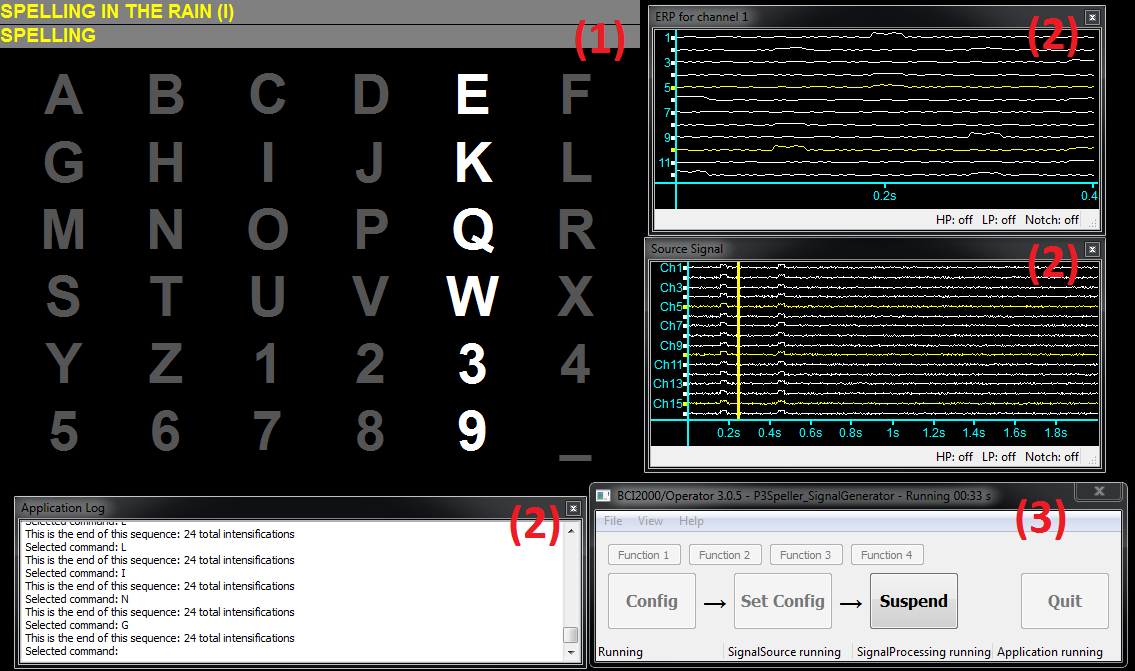
\includegraphics[scale=0.48]{images/P300SpellerBase.png}
\caption{Das Erscheinungsbild des ursprünglichen P300-Spellers (1) mit den dazugehorigen Monitor-Komponenten (2), sowie dem Operator-Modul (3).}
\label{P300SpellerComponents}
\end{center}
\end{figure}







\pagebreak

Die Realisierung erfordert eine Erweiterung des P300-Spellers um Funktionen, welche nachfolgend vereinfacht aufgeführt werden.
\begin{itemize}
\item Die Möglichkeit zur Darstellung des aktuellen Bildausschnitts im Hintergrund
\item Darstellung der Speller-Matrix in variabler Position, Größe und Typ
\item Änderung der Stimulus-Visualisierung von Buchstaben zu halb transparanten Zeilen bzw. Spalten
\item TCI/IP-Kommunikation zwischen Speller und Plugin
\item Durchführung der Stimulus Sequenzen auf Anfrage des Plugins\\
\end{itemize}

Um oben beschriebene Funktionen zu implementieren ist es erforderlich die Architektur des P300-Spellers bzw. des \acs{BCI2000}-Frameworks zu verstehen.\\
Abbildung \ref{ausfuehrungsGraph} zeigt den Ausführungsplan, gemäß der Reihenfolge wie die Ereignisse innerhalb des P300-Spellers auftreten.\\


\begin{figure}[h!]
\begin{center}
\begin{tikzpicture}[scale=1.05,
rectStart/.style={rectangle, draw=black!50, fill=black!10, minimum width=5mm, minimum height=10mm, text width=20mm, align=center, rounded corners},
rectWait/.style={rectangle, draw=black!50, fill=yellow!10, minimum width=5mm, minimum height=10mm, text width=40mm, align=center},
rectOnce/.style={rectangle, draw=black!50, fill=blue!10, minimum width=5mm, minimum height=10mm, text width=40mm, align=center},
rectLoop/.style={rectangle, draw=black!50, fill=green!10, minimum width=5mm, minimum height=10mm, text width=40mm, align=center},
rectTrigger/.style={rectangle, draw=black!50, fill=green!10, minimum width=5mm, minimum height=10mm, text width=40mm, align=center}
]

% StimulusTask Schleif, insofern sie für uns relevant ist, bzw rein zur Vorstellung

\node[rectStart] (OnStart) at (-2, 4) {Start};
\node[rectStart] (OnStop) at (2, 4) {Stop};
\node[rectWait] (OnPreSequence) at (0, 2.5) {OnPreSequence};
\node[rectOnce] (DoPreSequence) at (-3.598, 1.0) {DoPreSequence};
\node[rectOnce] (OnSequenceBegin) at (-3.598, -1.0) {OnSequenceBegin};
\node[rectLoop] (OnNextStimulusCode) at (0, -2.8) {OnNextStimulusCode}; % loop
\node[rectOnce] (DoPostSequence) at (3.598, -1.0) {DoPostSequence};
\node[rectOnce] (OnClassResult) at (3.598, 1.0) {OnClassResult};
\node[rectTrigger] (OnEnter) at (5.598, 2.5) {OnEnter};



\path[->] 	(OnStart) 				edge 					node {} (OnPreSequence)
			(OnPreSequence) 		edge 					node {} (OnStop)
			(OnClassResult) 		edge 					node {} (OnPreSequence)
			(OnPreSequence) 		edge 					node {} (DoPreSequence)
			(DoPreSequence) 		edge 					node {} (OnSequenceBegin)
			(OnSequenceBegin) 		edge 		 			node {} (OnNextStimulusCode)
			(OnNextStimulusCode) 	edge 		 			node {} (DoPostSequence)
			(DoPostSequence) 		edge 		  			node {} (OnClassResult)
			(OnNextStimulusCode) 	edge 		[loop below]node {} (OnNextStimulusCode)
			(OnClassResult) 		edge 					node {} (OnEnter);
			
\end{tikzpicture}
\caption{Die Ausführungsreihenfolge der internen Funktionen des P300-Spellers}
\label{ausfuehrungsGraph}
\end{center}
\end{figure}



Ausgehend davon das die Konfiguration und Initialisierung innerhalb des Startpunkts abgeschlossen ist, wird mit jedem Schleifen-Durchlauf beginnend bei \textit{OnPreSequence} eine Eingabe ermittelt.
Innerhalb der Schleife werden zunächst die Stimuli erstellt. 
Daraufhin beginnt die Eingabe-Ermittlung indem die Stimuli-Sequenz abgespielt wird, das heißt die Zeilen und Spalten der Speller-Matrix werden angezeigt und wieder ausgeblendet.
Dieser Vorgang entspricht in Abbildung \ref{ausfuehrungsGraph} der Rekursion des \textit{OnNextStimulusCode}-Blocks.
Nach Abschluss der Sequenz wird das resultierende Ergebnis ermittelt und weitergegeben.\\

Innerhalb der nächsten Seiten werden die einzelnen Entwicklungsabschnitte des AGS-P300-Spellers vorgestellt 
und mögliche Szenarien für die Implementierung betrachtet und bewertet. 
Basierend auf dieser Bewertung wird anschließend das zu realisierende Szenario ausgewählt.\\






\pagebreak
\subsection{Darstellung des Hintergrundbilds}
\vspace{0.3cm}

Die Einbindung des Hintergrunds ist ein relativ einfacher, aber sehr wichtiger Aspekt in der Umsetzung des Konzepts, da die Eingabe-Ermittlung außerhalb des Spiels durchgeführt wird.
Der Speller erhält das Bild des aktuellen Spielausschnitts, zeigt dieses im Hintergrund an und überlagert das Bild mit der aktuellen Speller-Matrix. 
Für diesen Zweck muss der Speller erweitert werden, da dieser über keine Möglichkeit zur Manipulation des Hintergrunds verfügt, 
da dies ursprünglich nur über die Textstimulus-Objekte erfolgt und unpraktisch für die Darstellung eines einzelnen Bildes ist.
In Abbildung \ref{bgGraph} wird der Vorgang dargestellt und relativ zu Abbildung \ref{ausfuehrungsGraph} eingeordnet.\\


\begin{figure}[h!]
\begin{center}
\begin{tikzpicture}[scale=1.0,
rectStartStop/.style={rectangle, draw=black!50, fill=black!10, minimum width=10mm, minimum height=7mm, text width=10mm, align=center, rounded corners},
rectDoPre/.style={rectangle, draw=black!50, fill=blue!10, minimum width=60mm, minimum height=50mm, text width=60mm, align=center},
rectDoPost/.style={rectangle, draw=black!50, fill=blue!10, minimum width=60mm, minimum height=50mm, text width=50mm, align=center},
rectStimulusCode/.style={rectangle, draw=black!50, fill=green!10, minimum width=5mm, minimum height=10mm, text width=40mm, align=center},
rect/.style={rectangle, draw=black!50, fill=green!10, minimum width=5mm, minimum height=10mm, text width=40mm, align=center},
rectVoid/.style={rectangle, draw=black!0, fill=black!0, minimum width=5mm, minimum height=10mm, text width=40mm, align=center}
]

\node[rectDoPre] (DoPreSequence) at (-4, 0) {};
\node[rectDoPost] (DoPostSequence) at (4, 0) {};

\node[rectStimulusCode] (OnNextStimulusCode) at (0, -3.5) {OnNextStimulusCode};


\node at (-5.5, 2) {DoPreSequence};

\node[rectStartStop] (prestart) at (-3, 1.75) {Start};
\node[rect] (image) at (-4, 0.65) {Setze Hintergrundbild};
\node[rect] (foreground) at (-4, -0.75) {Wechsle Prozess in Vordergrund};
\node[rectStartStop] (prestop) at (-3, -1.9) {Stop};



\node at (2.75, 2) {DoPostSequence};

\node[rectStartStop] (poststop) at (3, 1) {Stop};
\node[rect] (background) at (4, -0.25) {Wechsle Prozess in Hintergrund};
\node[rectStartStop] (poststart) at (3, -1.5) {Start};



\path[->] 	(prestart) 					edge 					node {} (image)
			(foreground) 				edge 					node {} (prestop)
			(image) 					edge 					node {} (foreground)
			(poststart) 				edge 					node {} (background)
			(background) 				edge 					node {} (poststop)
			(DoPreSequence) 			edge 					node {} (OnNextStimulusCode)
			(OnNextStimulusCode) 		edge 					node {} (DoPostSequence);



\end{tikzpicture}
\caption{Definition des aktuellen Hintergrunds und Fokussierung auf den Speller}
\label{bgGraph}
\end{center}
\end{figure}

Vor jeder Eingabe-Ermittlung wird das Bild in den Hintergrund des Spellers gesetzt. 
Anschließend ist es vor der Eingabe-Ermittlung erforderlich, dass der Prozess des Spellers in den Vordergrund verschoben wird.
So ersetzt der Speller für den Zeitraum der Eingabe-Ermittlung die Anzeige des Spiels. 
Nach Abschluss dieses Vorgangs wechselt der Speller-Prozess wieder zurück in den Hintergrund.\\





\pagebreak
\subsection{Konfiguration der Speller-Matrix}
\vspace{0.3cm}

Zunächst befassen wir uns mit der Frage, ob es eine Speller-Matrix sein muss oder ob eine andere Variante möglicherweise sinnvoller wäre.
Eine durchaus denkbare Alternative wäre hierfür beispielsweise, dass alle Interaktions-Objekte eines Bildausschnittes jeweils als einzelne Stimuli, 
statt als Zeile oder Spalte aus mehreren Stimuli, gezeigt oder verborgen werden. 
Die Stimuli-Visualisierung kann beispielsweise über das Aufleuchten eines der Objekte erfolgen.
Sofern die Stimuli ebenfalls in zufälliger Reihenfolge dargestellt werden und dem Oddball-Paradigma folgen, spricht auf den ersten Blick nichts gegen eine solche Alternative,
auf den zweiten Blick hingegen ergeben sich einige mögliche Probleme.
Das Oddball-Paradigma erfordert, dass immer eine Mindestmenge verschiedener Stimuli vorhanden ist.
Es entsprechend immer genügend Objekte geben muss oder "`Dummy"'-Objekte hinzugefügt werden müssten.
Weiterhin ist unklar in wie weit sich die Größe einzelner Objekte auf die Ergebnisse auswirken könnte, 
da unterschiedlich große Objekte unterschiedlich viel Aufmerksamkeit auf sich ziehen und entsprechend anders wahrgenommen werden könnten.
Damit wären die Bedinungen des Oddball-Paradigma's verletzt und dieses Szenario nicht mehr anzuwenden.
Sollte allerdings eine einheitliche Größe für alle Objekte gewählt werden können, dann muss zusätzlich gewährleistet werden, dass die Objekte sich nicht überlappen.
Da so \acs{P300 ERP}'s auch bei falschen Objekten ausgelöst werden könnten.\\

Folglich ergibt sich in Anbetracht der beschriebenen Alternative und den möglichen Problemen, dass es offenbar sinnvoll ist den Speller-Matrix-Ansatz weiterhin beizubehalten.\\


Für die Implementierung muss nun die Möglichkeit zur Definition variabler Speller-Matrizzen erarbeitet werden.
Da jede Eingabe-Ermittlung eine eigene Speller-Matrix bedingen kann, 
ist es sinnvoll nach Erhalt der Parameter diese an eine Methode zu übergeben, die die Speller-Matrix aufbaut.

In Abbildung \ref{spellermatrix} ist das Flussdiagramm zu sehen, das die Erstellung einer Speller-Matrix beschreibt.
Die für den Aufbau notwendigen Parameter sind die Position, die Größe und der Typ der Matrix.

\pagebreak 

\begin{figure}[h!]
\begin{center}
\begin{tikzpicture}[scale=0.9,
rectStart/.style={rectangle, draw=black!50, fill=black!10, minimum width=5mm, minimum height=10mm, text width=40mm, align=center, rounded corners},
rectDoWork/.style={rectangle, draw=black!50, fill=green!10, minimum width=5mm, minimum height=10mm, text width=40mm, align=center},
raute/.style={rectangle,rotate=45,draw=black!100,minimum width=20mm,minimum height=20mm, align=center},
rectText/.style={rectangle, draw=black!0, minimum width=5mm, minimum height=10mm, text width=20mm, align=center}]

\node[rectStart] (Start) at (0, 0) {Parameter erhalten};
\node[rectDoWork] (Matrix) at (-3, -1.6) {Erstelle Matrix-Rechteck};
\node[rectDoWork] (Elements) at (3, -1.6) {Berechne Größe der Stimuli-Elemente};
\node[rectDoWork] (Stimuli) at (0, -3.5) {Erstelle Stimulus-Objekt für jedes Matrix-Element};

%\node[rectText] at (0, -6.25) {Stimuli \\erstellt?};
%\node[raute] (check) at (0, -6.25) {};
%\node at (0.4, -8) {Ja};
%\node at (1.2, -4.9) {Nein};

\node[rectDoWork] (Assoziation) at (0, -5.7) {Assoziiere Stimuli-Objekte mit \\Zeilen und Spalten};
\node[rectStart] (Stop) at (0, -7.65) {Speller-Matrix erstellt};

\path[->] 	(Start) 				edge 					node {} (Matrix)
			(Start) 				edge 					node {} (Elements)
			(Elements) 				edge 					node {} (Stimuli)
			(Matrix) 				edge 					node {} (Stimuli)
			%(Stimuli) 				edge 	[bend right]	node {} (check)
			%(check) 				edge 	[bend right]	node {} (Stimuli)
			%(check) 				edge 					node {} (Assoziation)
			(Stimuli) 				edge 					node {} (Assoziation)
			(Assoziation) 			edge 					node {} (Stop);

\end{tikzpicture}
\caption{Das Flussdiagramm der Speller-Matrix-Erstellung}
\label{spellermatrix}
\end{center}
\end{figure}

Vor jeder neuen Eingabe-Ermittlung werden die damit verbundenen Parameter an die Methode zur Erstellung einer individuellen Speller-Matrix übergeben (zu sehen in Abbildung \ref{matrizzen}).
Anhand der Parameter wird das Rechteck der Speller-Matrix definiert und innerhalb der Anzeige positioniert.
Mit Hilfe des Typs der Matrix wird die Größe jedes Stimulus-Objekts berechnet, sodass über die Zeilen und Spalten iteriert werden kann, um für jedes Element ein Stimulus-Objekt zu erstellen.
Jedes dieser Objekte wird mit seiner entsprechenden Zeile und Spalte in einer Assoziations-Karte verknüpft, 
die für die Assoziation zwischen Stimulus und Signal verantwortlich ist.
Durch diese Verknüpfung kann schließlich das Ergebnis ermittelt werden.

\begin{figure}[ht]
\centering
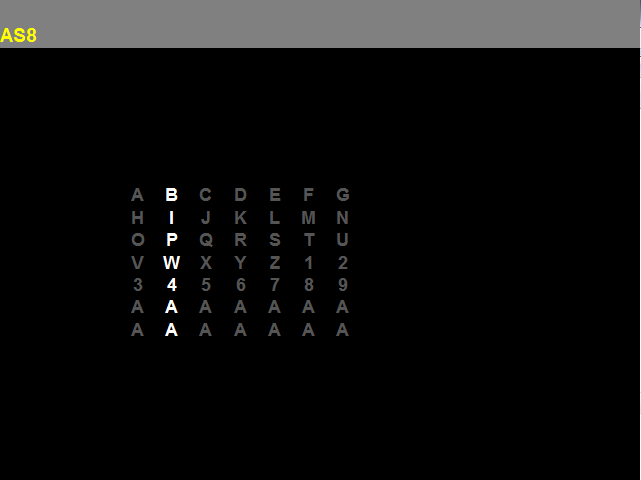
\includegraphics[scale=0.35]{images/customMatrix.png}
\caption{Eine dynamisch aufgebaute Speller-Matrix des Typs 7x7}
\label{matrizzen}
\end{figure}

Die Erstellung individueller Speller-Matrizen erfüllt weiterhin die Bedingungen des Oddball-Paradigmas, sofern der Typ der Matrix nicht zu klein gewählt wird.


















\pagebreak









\pagebreak
\subsection{Stimulus-Visualisierung}
\vspace{0.3cm}

Gemäß des letzten Kapitels wird weiterhin eine Speller-Matrix verwendet, 
jedoch ist die bisherige Darstellung der Stimuli via aufleuchtender Buchstaben für unsere Bedürfnisse nicht angemessen.
Deshalb ist die Entwicklung eines neuen Stimulus-Derivats erforderlich.
Eine wichtige Anforderung an die neuen Stimuli ist, dass sie einen Reiz unabhängig vom Inhalt erzeugen und somit vor jedem Hintergrundbild dargestellt werden können.\\

Für die Darstellung der Stimuli besteht zum einen die Möglichkeit die Ränder eines Matrix-Elements aufleuchten zu lassen, sodass der Inhalt weiterhin sichtbar ist.
Zum anderen kann die Fläche eines Matrix-Elements halb transparent mit Farbe gefüllt werden, so dass diese Farbe die Fläche überlagert und der Inhalt ebenso sichtbar bleibt.\\

Weiterhin muss jedoch die Anforderung beachtet werden, dass Speller-Matrizen mit beliebiger Position, Größe und Typ dargestellt werden können.
Daraus ergibt sich wie in Abbildung \ref{NoMesh} zu sehen ist, dass es dem Benutzer deutlich erschwert ist sich auf ein Matrix-Element zu fokussieren, wenn dessen Position unbekannt ist.
Eine Eingabe-Ermittlung wird durch diesen Umstand entsprechend erschwert, sodass es sinnvoll ist eine adequate Vorschau zu visualisieren.

\begin{figure}[h!]
\begin{center}
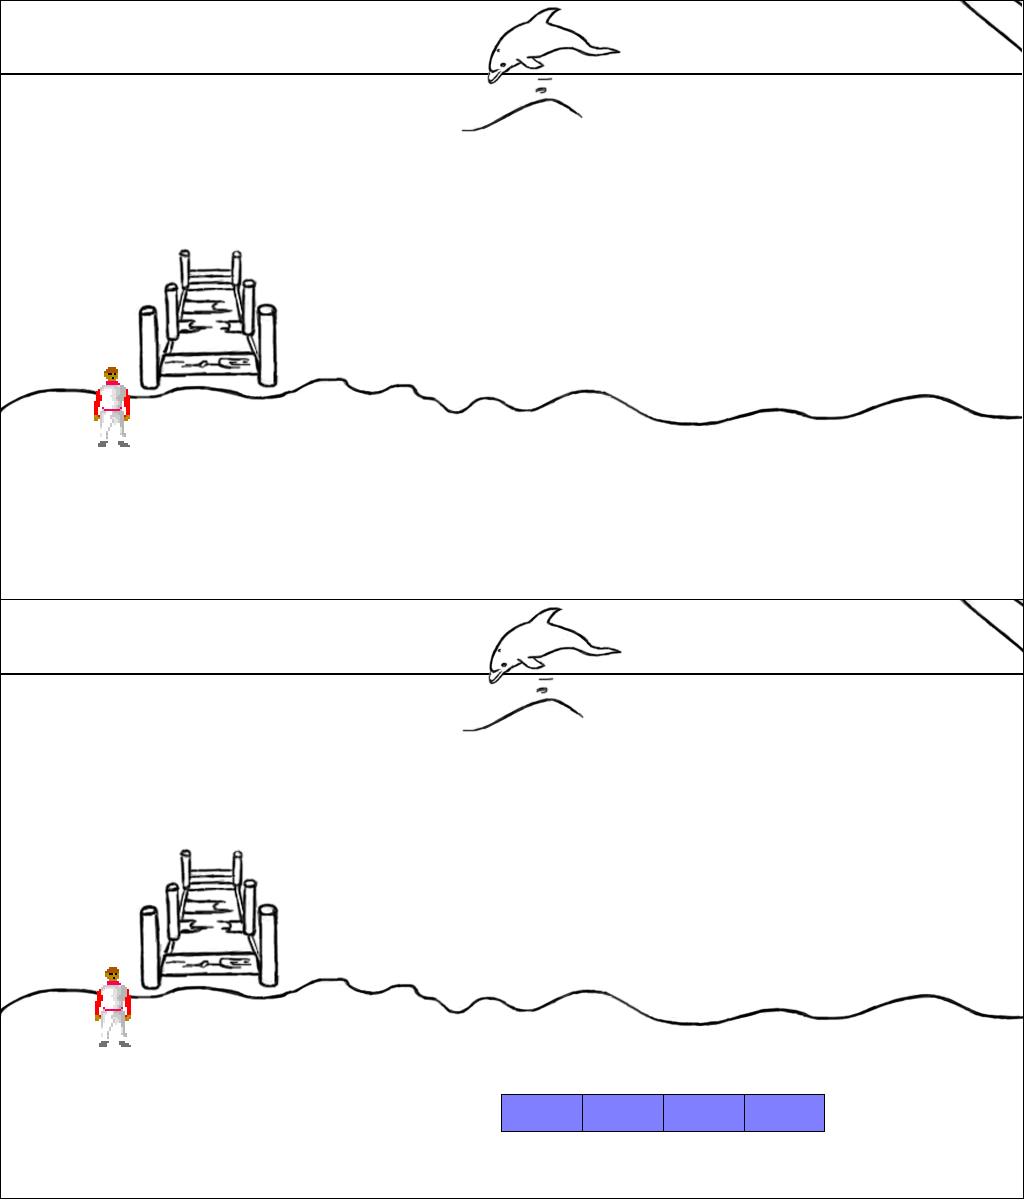
\includegraphics[scale=0.225]{images/NoMesh.png}
\caption{Stimuli-Visualisierung \textbf{ohne} Visualisierung der Speller-Matrix}
\label{NoMesh}
\end{center}
\end{figure}

\pagebreak

Abbildung \ref{Mesh} zeigt die gleiche Szene mit einer Visualisierung der Speller-Matrix.
Die Vorschau ermöglicht es einem Benutzer sich besser auf einen Bereich zu konzentrieren und erlaubt auch vorab den möglichen Eingabebereich besser zu lokalisieren.
Daher erscheint es sinngemäß eine solche Visualisierung auch in der Implementierung zu verwenden, da das Fehlen der Vorschau mit einer Tastatur ohne Tastenbeschriftung gleich käme.\\

\begin{figure}[h!]
\begin{center}
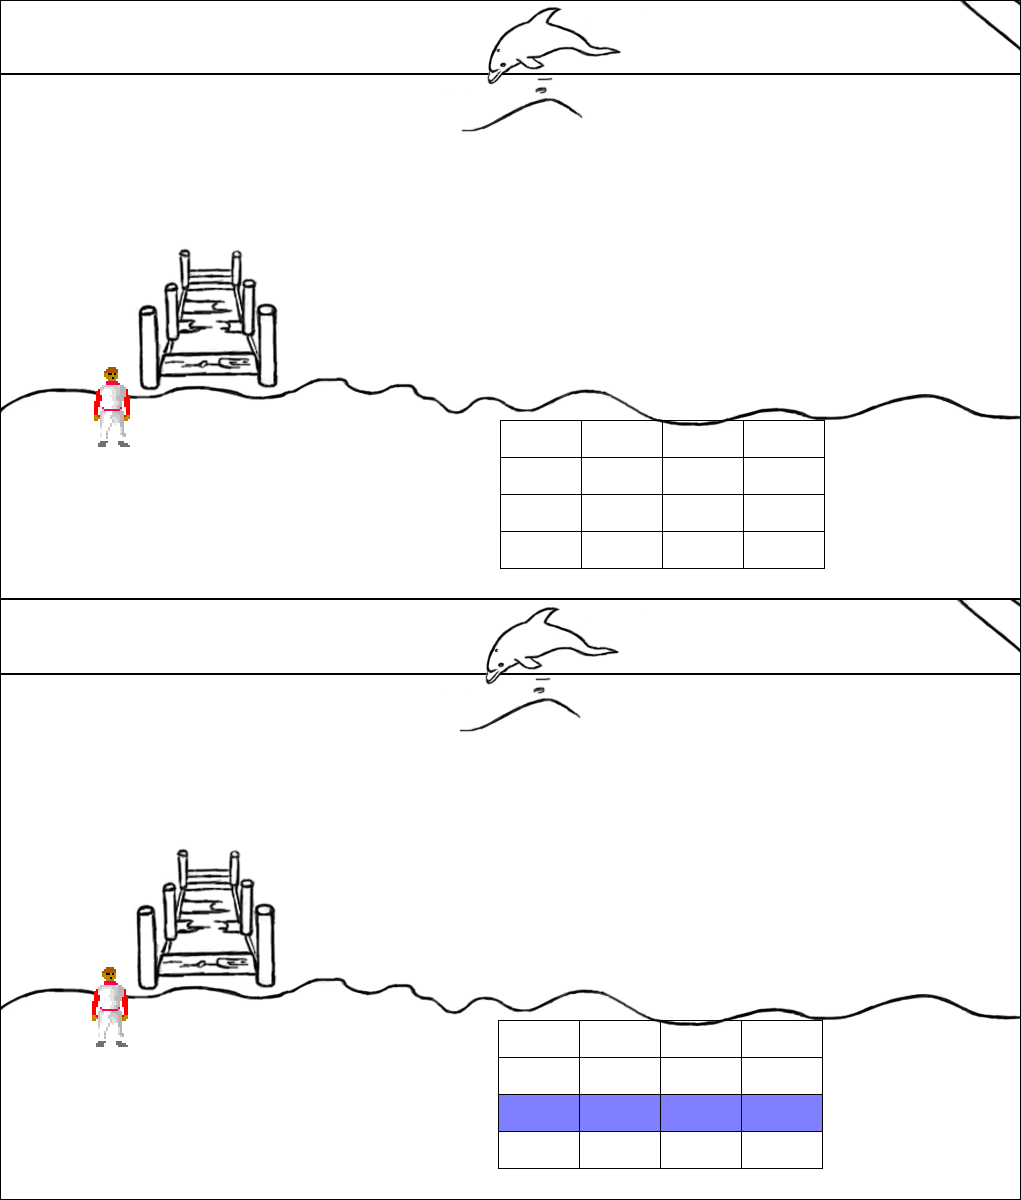
\includegraphics[scale=0.225]{images/Mesh.png}
\caption{Stimuli-Visualisierung \textbf{mit} Visualisierung der Speller-Matrix}
\label{Mesh}
\end{center}
\end{figure}

In Anbetracht der Tatsache, dass in der Implementierung die Matrix durch ein Raster visualisiert wird, 
ist die Darstellung der Stimuli durch aufleuchtende Rahmen möglicherweise nicht in der Lage ausreichend gut wahrgenommen zu werden.
Aus diesem Grund liegt es nahe, die Variante der farbüberlagernden Fläche zu verwenden, wie sie auch schon in den gezeigten Abbildungen verwendet wurde.

\pagebreak
\subsection{Speller-Plugin-Kommunikation}
\vspace{0.3cm}

Die Kommunikation zwischen Speller und Plugin wird ähnlich zu BCI2000 ebenfalls via TCP/IP durchgeführt.
Dabei nimmt der Speller die Rolle eines Servers ein, bei dem sich das Engine Plugin als Client anmelden muss.
In Abbildung \ref{spellerplugintcpip} wird der Ablauf der Kommunikation auf Seiten des Spellers dargestellt.\\

\begin{figure}[h!]
\begin{center}
\begin{tikzpicture}[scale=1.0,
rectStart/.style={rectangle, draw=black!50, fill=black!10, minimum width=5mm, minimum height=7mm, text width=10mm, align=center, rounded corners},
rectStart2/.style={rectangle, draw=black!50, fill=black!10, minimum width=5mm, minimum height=7mm, text width=20mm, align=center, rounded corners},
rectDoWork/.style={rectangle, draw=black!50, fill=green!5, minimum width=5mm, minimum height=10mm, text width=40mm, align=center},
rectOnPreSeq/.style={rectangle, draw=black!50, fill=blue!5, minimum width=70mm, minimum height=70mm, text width=70mm, align=center},
rectOnClassRes/.style={rectangle, draw=black!50, fill=blue!5, minimum width=60mm, minimum height=50mm, text width=70mm, align=center},
rectText/.style={minimum width=5mm, minimum height=10mm, text width=20mm, align=center},
rectText2/.style={minimum width=5mm, minimum height=5mm, text width=5mm, align=center}]

\node[rectStart2] (start) at (-3, 5.25) {Starte Server};
\node[rectStart2] (stop) at (3, 5.25) {Stoppe Server};
\node[rectText2] (dots1) at (0.5, 4) {...};
\node[rectText2] (dots2) at (0.5, -4) {...};

% OnPreSequence
\node[rectOnPreSeq] (OnPre) at (-4, 0) {};
\node[rectText] (OnSeqText) at (-6.4, 3) {Empfangen};

\node[rectStart] (OnPreStart) at (-1.5, 2.8) {Start};
\node[rectStart] (OnPreStop) at (-1.5, -2.8) {Stop};

\node[rectDoWork] (waitParams) at (-5, 1.9) {Warte auf Daten};
\node[rectDoWork] (receiveParams) at (-5, 0.5) {Empfange Matrix-Parameter};
\node[rectDoWork] (receiveImage) at (-5, -0.9) {Empfange Bild-Puffer};
\node[rectDoWork] (buildImage) at (-5, -2.3) {Rekonstruiere Bild aus Bild-Puffer};


% OnClassResult
\node[rectOnClassRes] (OnClass) at (4.25, 0) {};
\node[rectText] (OnClassText) at (7, 2.1) {Senden};
\node[rectStart] (OnClassStart) at (1.5, -1.8) {Start};
\node[rectStart] (OnClassStop) at (1.5, 1.8) {Stop};

\node[rectDoWork] (waitResult) at (4.5, -0.75) {Warte auf Ergebnis};
\node[rectDoWork] (sendResult) at (4.5, 0.75) {Sende Ergebnis};


 \path[->] 	 (dots1) 				edge 					node {} (OnPreStart)
			 (OnPreStop) 			edge 					node {} (dots2)
			 (dots2) 				edge 					node {} (OnClassStart)
			 (OnClassStop) 			edge 					node {} (dots1)			
			 (start) 			edge 					node {} (OnPreStart)		
			 (dots1) 			edge 					node {} (stop)				 
			 (OnPreStart) 			edge 		[bend right]node {} (waitParams)
			 (waitParams) 			edge 					node {} (receiveParams)
			 (receiveParams) 		edge 					node {} (receiveImage)		
			 (receiveImage) 		edge 					node {} (buildImage)
			 (buildImage) 			edge 		[bend right]node {} (OnPreStop)
			 (OnClassStart) 		edge 		[bend right]node {} (waitResult)
			 (waitResult) 			edge 					node {} (sendResult)			 
			 (sendResult) 			edge 		[bend right]node {} (OnClassStop);

\end{tikzpicture}
\caption{Die Ausführungsreihenfolge der TCP/IP-Kommunikation auf Seiten des AGS-P300-Spellers}
\label{spellerplugintcpip}
\end{center}
\end{figure}

Bei jeder Anfrage werden zunächst die Parameter der Speller-Matrix übertragen. 
Anschließend werden die Bild-Daten gepuffert und das Bild anhand der Daten rekonstruiert.
Sobald dieser Vorgang abgeschlossen ist werden die Parameter und das Bild weitergegeben, sodass der Speller fortfahren kann.\\

Nach Abschluss und Ermittlung der Eingabe wird das Ergebnis an das Plugin zurückgesendet und dort verarbeitet.
Der Speller wird während dieser Zeit auf eine erneute Anfrage des Spiels warten.









\pagebreak
\section{Das AGS-P300-Plugin}

Dieses Kapitel befasst sich mit der Entwicklung eines Engine Plugins und soll die Schnittstelle zwischen AGS-Spiel und Speller darstellen,
so dass die Kommunikation zwischen Spiel und Speller ermöglicht wird.\\

Aus diesem Grund ist der Funktionsumfang des Plugins im Vergleich zum Speller relativ gering, da lediglich die Daten aufbereitet, versendet und wieder empfangen werden müssen.\\
In Abbildung \ref{pluginPlan} werden die inneren und äußeren Abläufe aus Sicht des Plugins dargestellt.\\




\begin{figure}[h!]
\begin{center}
\begin{tikzpicture}[scale=1.0,
rectStart/.style={rectangle, draw=black!50, fill=black!10, minimum width=5mm, minimum height=7mm, text width=10mm, align=center, rounded corners},
rectStart2/.style={rectangle, draw=black!50, fill=black!10, minimum width=5mm, minimum height=7mm, text width=20mm, align=center, rounded corners},
rectDoWork/.style={rectangle, draw=black!50, fill=green!5, minimum width=5mm, minimum height=7mm, text width=40mm, align=center},
rectDoWork2/.style={rectangle, draw=black!50, fill=green!5, minimum width=5mm, minimum height=7mm, text width=25mm, align=center},
rectDoWorkSmall/.style={rectangle, draw=black!50, fill=green!5, minimum width=5mm, minimum height=7mm, text width=15mm, align=center},
rectMisc/.style={rectangle, draw=black!50, fill=yellow!25, minimum width=5mm, minimum height=7mm, text width=15mm, align=center},
rectPlugin/.style={rectangle, draw=black!50, fill=blue!5, minimum width=140mm, minimum height=70mm, text width=110mm, align=center},
rectText/.style={minimum width=5mm, minimum height=10mm, text width=40mm, align=center}]


\node[rectStart] (start) at (-3, 3) {Start};
\node[rectMisc] (spiel) at (0, 3) {Spiel};
\node[rectStart] (stop) at (3, 3) {Stop};

\node[rectDoWork] (request) at (-2.5, 1.25) {Stelle Anfrage};
\node[rectDoWork] (result) at (2.5, 1.25) {Gebe Ergebnis zurück};

\node[rectPlugin] (plugin) at (0, -3.5) {};
\node[rectText] (pluginText) at (0, -0.75) {AGS Engine Plugin};

\node[rectStart] (startPlugin) at (-3.5, -0.75) {Start};
\node[rectStart] (stopPlugin) at (3.5, -0.75) {Stop};


\node[rectMisc] (speller) at (0, -8) {Speller};

\node[rectDoWork] (params) at (-3.5, -2.5) {Bearbeite Parameter für Speller-Matrix};
\node[rectDoWork] (image) at (-3.5, -4.25) {Bereite Bildpuffer vor};
\node[rectDoWork] (send) at (-3.5, -5.9) {Sende Parameter \& Bild-Daten};
\node[rectDoWork2] (waitresult) at (3.5, -5.9) {Warte auf Ergebnis};
\node[rectDoWork2] (recvresult) at (3.5, -2.5) {Empfange Ergebnis};


 \path[->] 	(start) 				edge 					node {} (spiel)
			(spiel) 				edge 					node {} (request)
			(result) 				edge 					node {} (spiel)
			(request) 				edge 					node {} (startPlugin)
			(stopPlugin) 			edge 					node {} (result)
			(startPlugin) 			edge 					node {} (params)
			(params) 				edge 					node {} (image)
			(image) 				edge 					node {} (send)
			(send) 					edge 					node {} (speller)		
			(speller) 				edge 					node {} (waitresult)
			(waitresult) 			edge 		[loop right]node {} (waitresult)
			(waitresult) 			edge 					node {} (recvresult)			
			(recvresult) 			edge 					node {} (stopPlugin)			
			(spiel) 				edge 					node {} (stop);


\end{tikzpicture}
\caption{Der Ablauf einer Anfrage des Spiels an das AGS Engine Plugin und die damit verbundenen Schritt bis zur Rückgabe des Ergebnisses}
\label{pluginPlan}
\end{center}
\end{figure}

\pagebreak

Beim Starten des Spiels wird zunächst eine TCP/IP-Verbindung zum AGS-P300-Speller aufgebaut.
Da das Plugin den Clienten einer Client-Server-Kommunikation darstellt ist es notwendig, dass der Speller bereits gestartet ist und auf die Verbindung des Plugins wartet.
Von diesem Zeitpunkt an ist das Plugin bereit, Anfragen des Spiels weiterzuleiten.
Eine Anfrage erfolgt durch Aufrufen einer Methode innerhalb des Spiels.
Diese Methode erwartet die Parameter zum Aufspannen der Speller-Matrix.
Das Plugin wird die Daten zunächst für den Sende-Vorgang vorbereiten und anschließend die Bild-Daten des Spiels von der Engine abfragen.
An dieser Stelle ist es nötig die Farbkanal-Repräsentation der Bild-Daten in \acs{RGBA} umzuwandeln, da der aktuelle Spielausschnitt von der Engine hingegen in \acs{BGRA} bereitstellt wird.
Die vorbereiteten Daten werden anschließend an den Speller gesendet.
Das Plugin wartet daraufhin auf das Ergebnis, welches dem ausgewählten Matrix-Element entspricht.
Nach weiterreichen des Ergebnisses wartet das Plugin auf eine erneute Anfrage, um den Vorgang zu wiederholen.\\








\pagebreak
\section{Erstellung des Point\&Click Test-Spiels}

Nach der Entwicklung des Spellers und des Plugins ist es notwendig diese zu testen.
Daher wird nachfolgend ein kleines Test-Spiel entwickelt, um die entwickelten Funktionen zu überprüfen.
Wie im Konzept geschrieben wird es sich optisch an "`The Secret of Monkey Island "' anlehnen.\\

Zur Entwicklung des Spiels wird das Adventure Game Studio in der Version 3.3.0 verwendet.
Weiterhin wird das AGS Engine Plugin im Spiel referenziert und geladen, sodass dessen Funktionen zur Verfügung stehen.\\

Das Spiel-Szenario verwendet eine Strandkulisse, die in Abbildung\footnote[1]{Bild-Quelle: \cite{JM2014}} \ref{strand1} zu sehen ist.
Sie wird im Hintergrund des Spiels dargestellt und je eine Hälfte bildet einen "`Raum"' bzw. eine Szene ab.\\

\begin{figure}[ht]
\centering
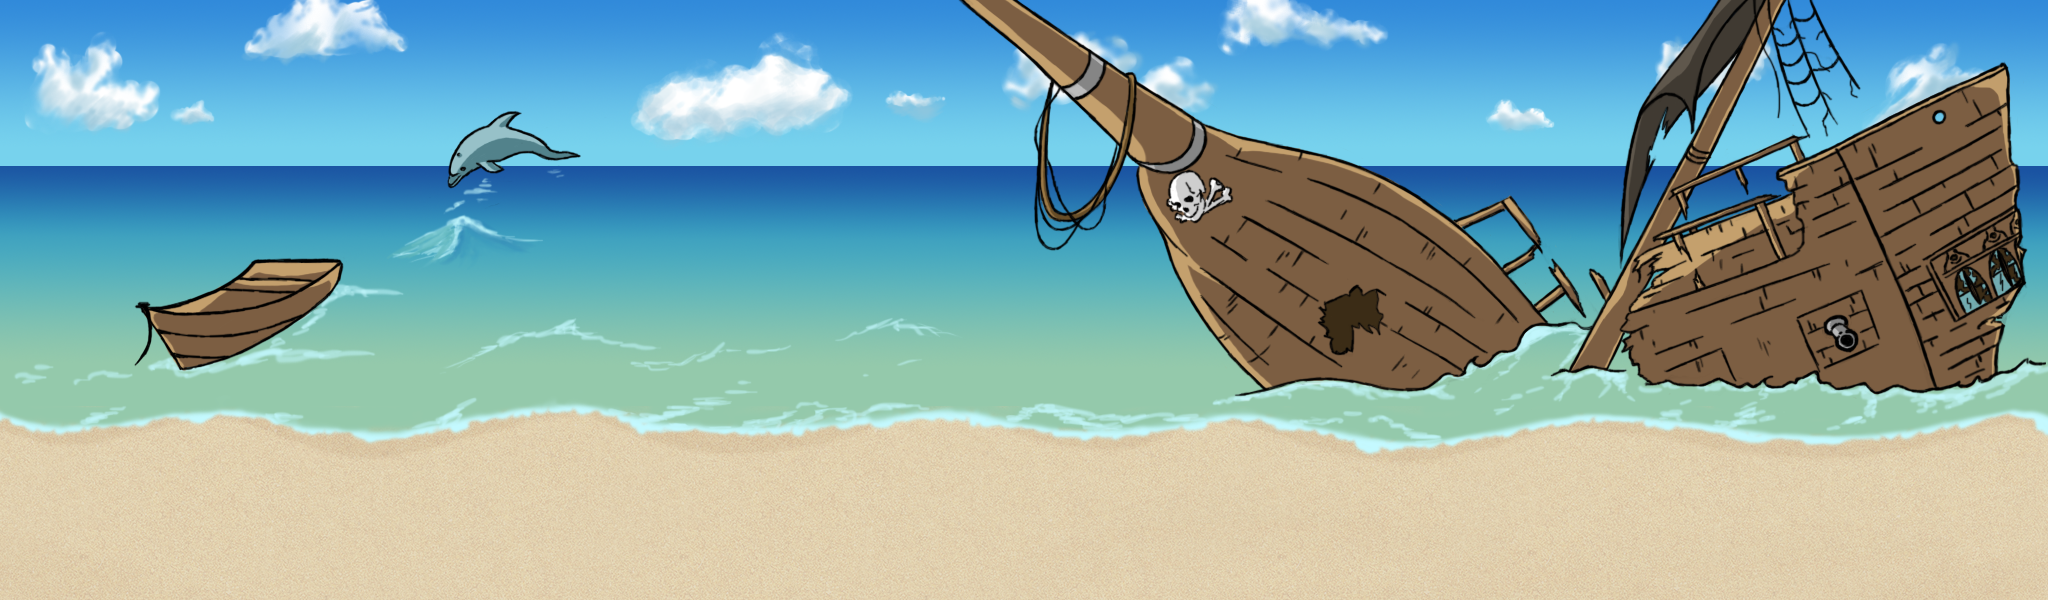
\includegraphics[scale=0.88]{images/MI_beach.png}
\caption{Die Strandkulisse des Test-Spiels}
\label{strand1}
\end{figure}

Während des Spiels soll eine Spielfigur über einen Strand bewegt werden, um Gegenstände auf dem Strand aufzuheben oder die Szenen zu wechseln.
Die Steuerung erfolgt hierbei über zwei Eingabe-Ermittlungen des Spellers.
Die erste ermittelt den auszuführenden Befehl, die zweite das Ziel des Befehls.
Bei der Befehlsauswahl kann es bei einer falschen Auswahl dazu kommen, dass ein Matrix-Element ausgewählt wird, dem kein Befehl zugeordnet ist. 
In einem solchen Fall wird die Befehlsauswahl wiederholt.\\

\pagebreak

Die notwendige Mindestgröße der Speller-Matrix sorgt bei der Befehlsauswahl dafür, 
dass die einzelnen Befehle mit mehreren Zeilen überlagert werden, 
um so dem Oddball-Paradigma zu entsprechen (siehe Abbildung \ref{Befehlsauswahl}).
Dies führt dazu, dass ein Befehl von mehreren Matrix-Elementen abgedeckt wird und ein Befehl demzufolge bei mehreren Speller-Ergenissen ausgewählt werden kann.\\

\begin{figure}[ht]
\centering
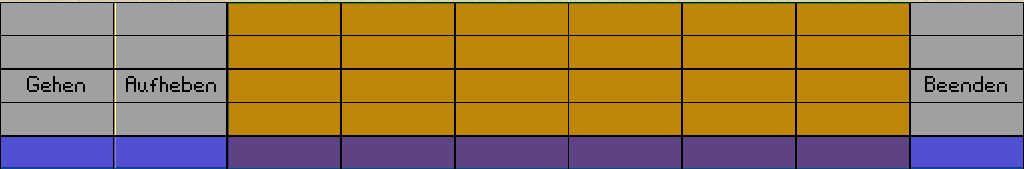
\includegraphics[scale=0.5]{images/Befehlsauswahl.png}
\caption{Die Befehlsauswahl des Test-Spiels}
\label{Befehlsauswahl}
\end{figure}

Bei der Zielauswahl gilt es ebenfalls eine Mindestgröße einzuhalten.
Allerdings ist es ebenfalls sinnvoll die Größe der Speller-Matrix zu begrenzen, da zu kleine Matrix-Elemente deren Fokussierung erschweren.
Zusätzlich würde dies einem Benutzer erhöhte Konzentration abverlangen und birgt die Gefahr, dass Ergebnisse negativ beeinflusst werden.
In Abbildung \ref{Zielauswahl} wird die Speller-Matrix der Zielauswahl dargestellt, die den gesamten begehbaren Bereich des Spiels umfasst.
Die drei in dieser Szene einzusammelnden Objekte sind ebenfalls zu sehen.\\


\begin{figure}[ht]
\centering
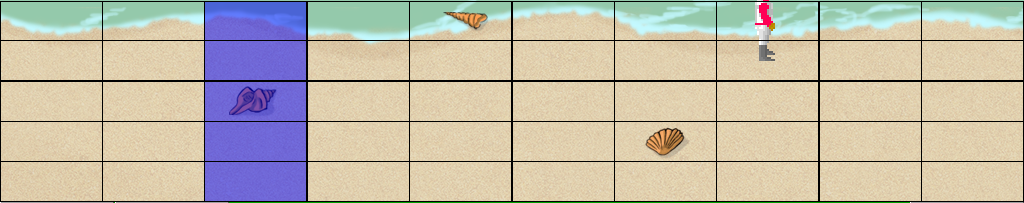
\includegraphics[scale=0.5]{images/Zielauswahl.png}
\caption{Die Zielauswahl des Test-Spiels}
\label{Zielauswahl}
\end{figure}

Mit Hinblick auf die Tests wurde das Spiel mit zwei Szenen und insgesamt sechs Objekten ausgestattet.
Es gibt drei Befehle "`Gehen"', "`Aufheben"' und "`Beenden"'.\\
Mit "`Gehen"' bewegt sich die Spielfigur an die ausgewählte Position. 
Um die Szene zu wechseln ist es beispielsweise erforderlich an den Rand der aktuellen Szene zu gehen.
Mit "`Aufheben"' bewegt sich die Spielfigur nur dann zum ausgewählten Feld, wenn sich dort ein Gegenstand befindet und hebt diesen dann auf, andernfalls würde eine Sprechblase erscheinen, dass es dort nichts aufzuheben gibt. \\
Der "`Beenden"'-Befehl beendet das Spiel, sofern dieser zwei mal in Folge ausgewählt wurde, andernfalls könnte das Spiel versehentlich bei einer falschen Eingabe beendet werden.\\

Das Aufheben eines Objekts und das Wechseln der Szene ist jeweils mit zwei Eingaben verbunden.
Daraus ergibt sich, dass das Spiel in insgesamt 14 Eingabe-Ermittlungen beendet ist, sofern eine Genauigkeit von 100\% vorliegt.




















    % 5b ) Tests
	\chapter{Tests}

In diesem Kapitel wird das Konzept des Tests beschrieben, da die Korrektheit der Erweiterung anhand von Tests verifiziert werden soll.
Die damit verbundenen Parameter und Abläufe werden in den nächsten Seiten festgehalten.


\section{Der Test-Plan}

Um zu verifizieren, dass die in dieser Masterarbeit entwickelte BCI-Erweiterung funktioniert, muss diese getestet werden.
Nachfolgend werden die einzelnen Bestandteile des Tests aufgeführt, die im Laufe dieses Kapitels genauer definiert 
und in einen sinnvollen Zusammenhang gebracht werden.

\begin{itemize}
\item Einführung zum Testablaufs und Einverständniserklärung
\item Fragebögen zur Ermittlung relevanter Informationen
\item Kalibrierung des BCI mittels P300-Speller
\item Vorher-Test der Kalibrierung
\item Durchführung des Test-Spiels mit dem AGS-P300-Speller
\item Nachher-Test der Kalibrierung
\item Ermittlung der subjektiven Belastung\\
\end{itemize}


\subsubsection{Ablauf des Tests}

Zu Beginn wird jeder Testperson der Ablauf des Tests erklärt.
Sollte eine Person allergisch auf Kontaktlinsenflüssigkeit sein, dann wäre der Test an dieser Stelle beendet, da diese zum Befeuchten der Elektroden verwendet wird.
Ansonsten wird jeder Proband gebeten eine Einverständniserklärung für die anonyme Verwendung der Daten innerhalb dieser Arbeit zu unterzeichnen.\\

Sobald der Test beginnen kann, muss zunächst ein Fragebogen ausgefüllt werden.
Dieser sammelt relevante Daten zur Einordnung der Testpersonen.
Anschließend beginnt die Kalibrierung des Emotiv EPOC mit Hilfe des P300-Spellers.
Sobald das BCI kalibriert ist werden der "`Vorher-Test"', das Test-Spiel und der "`Nacher-Test"' durchgeführt.
Vor der Kalibrierung und dem Test-Spiel, sowie vor und nach dem "`Nachher-Test"' wird jeweils ein kurzer Fragebogen ausgefüllt, der das Befinden der Testpersonen festhält.
Dies ist der Tatsache geschuldet, dass eine Verschlechterung der Ergebnisse auf Ermüdung durch die ungewohnte Belastung zurückgeführt werden könnte.
Nach dem Ausfüllen des letzten Fragebogens ist der Test abgeschlossen.
Alle verwendeten Fragebögen finden sich im Anhang ab Seite \pageref{anhang}.\\



\subsubsection{Kalibrierung des \acs{BCI}'s}

Bevor die einzelnen Speller-Tests beginnen können, muss das \acs{BCI} kalibriert werden.
Zu diesem Zweck muss jeder Probant zunächst die beiden Wörter \mbox{"`BRAIN"'} und \mbox{"`ISLAND"'} mit dem P300-Speller schreiben.
Die für die Kalibrierung und die Tests erforderlichen Testparameter wurden zuvor durch einzelne Tests mit einer geübten und einer ungeübten Testperson ermittelt.
Die daraus hervorgehenden Parameter wurden insbesondere in Bezug auf ungeübte Personen ausgewählt, 
da die Mehrheit der Testpersonen erwartungsgemäß keine Erfahrung im Umgang mit \acs{BCI}s vorweisen können.
\begin{itemize}
\item PreSequenceDuration: 2000ms
\item PostSequenceDuration: 2000ms
\item StimulusDuration: 125ms
\item InterStimulusDuration: 125-250ms
\item NumberOfSequences: 10 \\
\end{itemize}
Diese Parameter bestimmen die Wartezeit vor und nach jeder Stimuli-Sequenz, der Zeit \mbox{einer} Stimuli-Visualisierung und der Zeit zwischen zwei Stimuli-Visualisierungen.
Die Wartezeit zwischen den Sequenzen ist bewusst auf einem etwas höheren Wert festgelegt, da die Testpersonen den neuen Buchstaben vor der nächsten Sequenz finden und fokussieren müssen.
Die Dauer einer Sequenz beträgt das zehnfache der einfachen Sequenz, so dass jede Zeile bzw. Spalte zehn mal hervorgehoben wird.
Anhand der dadurch ermittelten Daten wird eine Klassifizierung mit dem "`P300-Classifier"' des BCI2000-Frameworks durchgeführt, 
die Klassifizierung führt hierfür eine \ac{SWLDA} durch \cite[S.208ff]{schalk2010practical}.
Dieser generiert Parameter die vom Speller geladen werden müssen, um individuelle Unterschiede der Probanden zu berücksichtigen.
Im Anschluss daran wird der Referenz-Test 1 durchgeführt.




\subsubsection{Referenz-Test 1 \& 2}
Bei der Verwendung von \acs{BCI}'s kann die Qualität der Ergebnisse je nach Individuum stark variieren.
Aus diesem Grund werden die Parameter der Klassifizierung im Referenz-Test 1 angewendet, um Aussagen über die relative Genauigkeit zu erhalten.
Um die Ergebnisse des Test-Spiels einordnen zu können wird ein zusätzlicher Referenz-Test 2 nach dem Test-Spiel durchgeführt.
Dieser ist vom Aufbau her äquivalent zum Referenz-Test 1.
Beide Tests dienen als Vergleichsreferenz für das Test-Spiel.\\

Um zu zeigen, dass die BCI-Erweiterung korrekt funktioniert, müssen die Ergebnisse des Test-Spiels eine ähnliche Genauigkeit wie Referenz-Test 1 besitzen.
Sollten die Ergebnisse hingegen schlechter sein, muss Referenz-Test 2 zum Vergleich hinzugezogen werden.
Auf diese Weise kann eine mögliche Ermüdung des Nutzers gezeigt oder ausgeschlossen werden.\\



\subsubsection{Durchführung des Test-Spiels}

Während des Test-Spiels müssen die Probanden mit der Spielfigur alle Objekte im Spiel aufheben, die Szene nach rechts wechseln und alle dort verbliebenen Objekte aufheben.
Jedes richtig ausgewählte Matrix-Element ist ein Treffer, jedes falsch ausgewählte ein Fehler. 
Die Befehle werden jeweils in einer Spalte durch fünf verschiedene Matrix-Elemente repräsentiert, daher haben die Probanden die Anweisung immer das mittlere Element auszuwählen, 
weil dieses den Schriftzug des Befehls enthält.
Die korrekte Spalte bei falscher Zeile würde den richtigen Befehl auswählen, jedoch trotzdem als Fehler bewertet werden.
In Abbildung \ref{befehlsmatrix} ist dies beispielhaft für die Auswahl des Befehls "`Aufheben"' dargestellt.\\

\pagebreak

\begin{figure}[h!]
\begin{center}
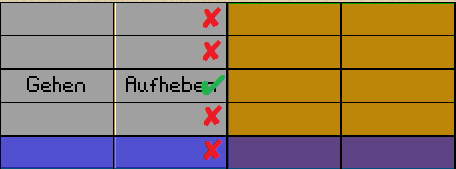
\includegraphics[scale=0.65]{images/BefehlsauswahlHitMiss.png}
\caption{Ein Ausschnitt der Speller-Matrix der Befehlsleiste. Die fünf Felder der Spalte \textit{Aufheben} wählen alle den selben Befehl aus, jedoch wird nur das Feld mit dem grünen Hakens als Treffer gewertet.}
\label{befehlsmatrix}
\end{center}
\end{figure}


Das Spiel wird beendet, sobald alle Objekte aufgehoben sind oder 25 Eingabe-Ermittlungen erreicht sind.
Die relative Genauigkeit jeder Testperson wird am Ende anhand der Treffer und Fehler ermittelt.
Das Ergebnis kann im Anschluss mit den Referenz-Tests verglichen und bewertet werden.\\



\subsubsection{Der NASA Task Load Index}
Im Anschluss an den gesamten Test muss jede der Testpersonen einen weiteren Fragebogen ausfüllen.
Dieser sogenannte \ac{NASA-TLX} \cite{hart1988development} umfasst sechs multidimensionale Bewertungen anhand derer eine subjektive Gesamtbelastung errechnet wird.
Die Bewertungen sind nachfolgend aufgeführt.

\begin{itemize}
\item Geistige Anforderungen
\item Körperliche Anforderungen
\item Zeitliche Anforderungen
\item Aufgabenerfüllung
\item Anstrengung
\item Frustration \\
\end{itemize}

Die ersten drei Punkte beziehen sich in erster Linie auf die Testperson, während die letzten drei Punkte die Durchführung der Aufgabe einbeziehen.
Die Erläuterungen der einzelnen Bewertungskriterien sind in Tabelle \ref{table:nasatlx} kurz dargestellt.

\begin{center}
\begin{table}[h!]
    \begin{tabular}{ | l | l | p{6cm} |}
    \hline
	\rule{0pt}{4ex} 
	\textbf{Bewertung} & \textbf{Skala} & \textbf{Erläuterung} \\ \hline 
	\rule{0pt}{4ex} 
    Geistige Anforderungen & gering/hoch & Wie gering/hoch war die geistige Beanspruchung? \\ \hline 
	\rule{0pt}{4ex} 
    Körperliche Anforderungen & gering/hoch & Wie gering/hoch war die körperliche Belastung?  \\ \hline
	\rule{0pt}{4ex} 
    Zeitliche Anforderungen & gering/hoch & Wie hoch war der zeitliche Druck? \\ \hline
	\rule{0pt}{4ex} 
    Aufgabenerfüllung & gut/schlecht & Wie gut empfand die Testperson ihr Ergebnis? \\ \hline
	\rule{0pt}{4ex} 
	Anstrengung & gering/hoch & Wie anstrengend war die Aufgabe für die Testperson? \\ \hline
	\rule{0pt}{4ex} 
	Frustration & gering/hoch & Wie frustierend war die Aufgabe für die Testperson? \\ \hline

	\end{tabular}
\caption{Die Bewertungskriterien des \acs{NASA-TLX}}
\label{table:nasatlx}
\end{table}
\end{center}

\pagebreak
Um die subjektive Gesamtbelastung zu berechnen wird zunächst die Gewichtung der Beanspruchungsstruktur ermittelt.
Dabei werden die einzelnen Bewertungskriterien gegenübergestellt, sodass die Testperson das jeweils ihrer Meinung nach wichtigere auswählt.
Im nächsten Schritt muss jedes Kriteriums anhand der Skala in Tabelle \ref{table:nasatlx} eingeordnet werden, um eine Wertung ablesen zu können.
Die Wertungen und Gewichtungen werden miteinander verrechnet, sodass sich eine durschnittliche Gesamtbelastung ergibt.
Die deutsche Fassung der \acs{NASA-TLX}-Fragebögen \cite{seifert02} befinden sich im Anhang dieser Arbeit.\\





%   Da die Aufzeichnung der \acs{P300 ERP}'s mittels des von der Universität bereitgestellten Emotiv EPOC durchgeführt werden.
%   P3,P4,PO8,Fz,Cz,Pz,PO7,Oz http://www.bci2000.org/phpbb/viewtopic.php?t=390





	
    % 6) Ergebnisse - Zusammenfassung der Ergebnisse und deren Bewertung
	\chapter{Ergebnisse}

In diesem Kapitel werden die Ergebnisse der Tests vorgestellt und in geeigneter Weise interpretiert.\\
Der gesamte Testablauf dauerte für jede Person etwa eine Stunde. 

Von insgesamt zehn Probanden waren nur sechs in der Lage den Test komplett durchzuführen und verwertbare Ergebnisse zu liefern.
Von den vier ausgeschlossenen Testpersonen erreichten zwei nur eine unzureichende Signalstärke.
Die dritte Person durfte am Test auf Grund von Epilepsie nicht teilnehmen.
Bei der vierten Testperson musste der Test auf Grund von Konzentrationsschwierigkeiten abgebrochen werden.\\


% Definition von Hit, Semi und Miss für den nachfolgenden Kontext

In Bezug auf die Tests und die Ergebnisse ist anzumerken, dass jede Ermittlung eines Zielfelds genau genommen aus der Kombination zweier Eingabe-Ermittlungen hervor geht.
Eine Auswahl setzt sich daher aus der ermittelten Zeile und der ermittelten Spalte zusammen.
Demzufolge müssen für die Interpretation der Ergebnisse zunächst drei Begriffe definiert werden, die ein ermitteltes Ergebnis beschreiben.

 \begin{Def} - \textbf{Hit} \\
 Wir sprechen von einem Hit, wenn eine richtig ermittelte Zeile mit einer richtig ermittelten Spalte kombiniert und somit das korrekte Zielfeld wiedergegeben wird.
 \end{Def}
 \begin{Def} - \textbf{Semi} \\
 Ein Semi tritt immer dann auf, wenn lediglich eine Zeile bzw. Spalte richtig und die andere falsch ermittelt wurde.
 \end{Def} 
 \begin{Def} - \textbf{Miss} \\
Ein Miss entspricht der Kombination aus je einer falsch ermittelten Zeile und Spalte.\\
 \end{Def}

 
Die Wahrscheinlichkeiten einer zufälligen Auswahl der Ergebnisse ist für die Referenz-Tests in Tabelle \ref{tab:randomReference} und für das Test-Spiel in Tabelle \ref{tab:randomGame} zu sehen.
In Bezug auf das Test-Spiel gibt es zwei Speller-Matrizen der Größen 5x9 und 5x10.
Zur Vereinfachung wird nur die Wahrscheinlichkeitsverteilung der 5x9-Speller-Matrix zum Vergleich herangezogen, 
da diese die meisten Eingabe-Ermittlungen vorzuweisen hat, darüberhinaus unterscheidet sich die Wahrscheinlichkeitsverteilung der 5x10-Speller-Matrix (dargestellt in Klammern) nur geringfügig von der 5x9-Speller-Matrix.


\begin{table}[h!]
\centering
\footnotesize{
\setlength{\extrarowheight}{5pt}
\begin{tabular}{|ccc|}
\multicolumn{3}{c}{6x6-Speller-Matrix} \\ \hline
\textbf{Hit} & \textbf{Semi} & \textbf{Miss} \\ \hline
2.77\% & 27.77\% & 69.44\% \\ \hline
\end{tabular}}
\caption{Die Wahrscheinlichkeitsverteilung der Referenz-Tests}
\label{tab:randomReference}
\end{table}



\begin{table}[h!]
\centering
\footnotesize{
\setlength{\extrarowheight}{5pt}
\begin{tabular}{|ccc|}
\multicolumn{3}{c}{5x9(5x10)-Speller-Matrix} \\ \hline
\textbf{Hit} & \textbf{Semi} & \textbf{Miss} \\ \hline
2.22\% (2.0\%)& 26.66\% (26.0\%)& 71.11\% (72.0\%) \\ \hline
\end{tabular}}
\caption{Die Wahrscheinlichkeitsverteilung des Test-Spiels}
\label{tab:randomGame}
\end{table}



In Tabelle \ref{tab:Ergebnisse} sind die Testergebnisse der einzelnen Testabschnitte jedes Probanden zu sehen.



\begin{table}[h!]
\centering
\footnotesize{
\setlength{\extrarowheight}{5pt}
\begin{tabular}{cc|ccc|ccc|ccc|}


\multicolumn{2}{c}{}			& \multicolumn{3}{c}{Referenz-Test 1} &	\multicolumn{3}{c}{Test-Spiel} & \multicolumn{3}{c}{Referenz-Test 2} 			\\
\multicolumn{1}{l}{TestNr.}	& \multicolumn{1}{c}{} 			& \multicolumn{1}{c}{\textbf{Hit}}	& \textbf{Semi}	& \multicolumn{1}{c}{\textbf{Miss}}	& \multicolumn{1}{c}{\textbf{Hit}}	& \textbf{Semi}	&\multicolumn{1}{c}{\textbf{Miss}} & \multicolumn{1}{c}{\textbf{Hit}}	& \textbf{Semi}	& \multicolumn{1}{c}{\textbf{Miss}}		\\ \cline{3-11}
\multirow{2}{*}{\textbf{01}}	&	\textbf{\#}	& 6		& 4		& 1		& 6		& 12	& 7		& 7		& 2		& 2		\\
								&	\%			& 54.5\%& 36.4\%& 9.1\%	& 24.0\%& 48.0\%& 28.0\%& 63.6\%& 18.2\%& 18.2\%\\ \cline{3-11}

\multirow{2}{*}{\textbf{02}}	&	\textbf{\#}	& 5		& 5		& 1		& 8		& 12	& 5		& 6		& 4		& 1		\\
								&	\%			& 45.5\%& 45.5\%& 9.1\%	& 32.0\%& 48.0\%& 20.3\%& 54.5\%& 36.4\%	& 9.1\%		\\ \cline{3-11}

\multirow{2}{*}{\textbf{03}}	&	\textbf{\#}	& 8		& 3		& 0		& 4		& 16	& 5		& 7		& 3		& 1		\\
								&	\%			& 72.7\%& 27.3\%& 0.3\%& 16.0\%& 64.0\%& 20.3\%& 63.6\%& 27.3\%& 9.1\% \\ \cline{3-11}

\multirow{2}{*}{\textbf{06}}	&	\textbf{\#}	& 8& 2& 1& 5& 10& 10& 2& 7& 2\\
								&	\%			& 72.7\%& 18.2\%& 9.1\%& 20.3\%& 40.3\%& 40.3\%& 18.2\%& 63.6\%& 18.2\%\\ \cline{3-11}

\multirow{2}{*}{\textbf{08}}	&	\textbf{\#}	& 4& 6& 1& 3& 15& 7& 4& 4& 3\\
								&	\%			& 36.4\%& 54.5\%& 9.1\%& 12.0\%& 60.3\%& 28.0\%& 36.4\%& 36.4\%& 27.3\%\\ \cline{3-11}

\multirow{2}{*}{\textbf{10}}	&	\textbf{\#}	& 6& 3& 2& 1& 11& 13& 7& 3& 1\\
								&	\%			& 54.5\%& 27.3\%& 18.2\%& 4.0\%& 44.0\%& 52.0\%& 63.6\%& 27.3\%& 9.1\%\\ \cline{3-11}	

								
								

%									\\ \cline{3-11}													
% TOTAL
%\multirow{2}{*}{\textbf{Total}}	&	\textbf{\#}	& 37& 23& 6& 27& 76& 47& 33& 23& 10 \\ 
%								&	\textbf{\%} & 56.1\%& 34.8\%& 9.1\%& 18.0\%& 50.7\%& 31.3\%& 50.0\%& 34.8\%& 15.2\% \\ \cline{3-11}
							

\end{tabular}
}
\caption{Die Ergebnisse der Tests}
\label{tab:Ergebnisse}

\end{table}


\pagebreak

In Tabelle \ref{tab:Ergebnisse} ist deutlich zu sehen, dass es sich bei den Eingabe-Ermittlungen der Referenz-Tests und des Test-Spiels nicht um zufällige Ergebnisse handelt,
da diese sich doch erheblich von den Wahrscheinlichkeitsverteilungen in den Tabellen \ref{tab:randomReference} und \ref{tab:randomGame} unterscheiden.

Eine Besonderheit stellen jedoch die vergleichsweise schlechten Ergebnisse von Testperson 10 dar, 
da diese als einzige Erfahrung im Umgang mit \acs{BCI}'s vorweisen konnte und bereits in früheren Stadien der \acs{BCI}-Erweiterung als Testperson fungierte.
Die damaligen Tests wurden jedoch mit einer \textit{StimulusDuration} und \textit{InterStimulusDuration} von jeweils 62.5ms, 
statt der im Test verwendeten 125ms und 125-250ms, durchgeführt und erzielten deutlich bessere Ergebnisse.
Allerdings sind diese Daten unzureichend, um weitere Schlüsse daraus zu ziehen, 
jedoch kann es sinnvoll sein für einzelne \acs{BCI}-Benutzer individuelle \textit{StimulusDuration}- und \mbox{\textit{InterStimulusDuration}}-Werte zu ermitteln, 
um die Genauigkeit weiter zu steigern.\\




\begin{table}[h!]
\centering
\footnotesize{
\begin{tabular}{|p{0.3cm} p{0.5cm}|		>{\columncolor[rgb]{0.84,.95,0.73}}p{0.3cm} >{\columncolor[rgb]{0.84,.95,0.73}}p{0.5cm}| 		p{0.3cm} p{0.5cm}| 		p{0.3cm} p{0.5cm}| 		p{0.3cm} p{0.5cm}| p{0.3cm} p{0.5cm}| p{0.3cm} p{0.5cm}| p{0.3cm} p{0.5cm}| p{0.3cm} p{0.5cm}|}
\hline
\tabbox{1} & \tabbox[b]{\LARGE{1}} &
\tabbox{2} & \tabbox[b]{\LARGE{5}} &
\tabbox{3} & \tabbox[b]{\LARGE{}} &
\tabbox{4} & \tabbox[b]{\LARGE{5}} &
\tabbox{5} & \tabbox[b]{\LARGE{}} &
\tabbox{6} & \tabbox[b]{\LARGE{}} &
\tabbox{7} & \tabbox[b]{\LARGE{2}} &
\tabbox{8} & \tabbox[b]{\LARGE{2}} &
\tabbox{9} & \tabbox[b]{\LARGE{}} \\ \hline

\tabbox{10} & \tabbox[b]{\LARGE{2}} &
\tabbox{11} & \tabbox[b]{\LARGE{6}} &
\tabbox{12} & \tabbox[b]{\LARGE{2}} &
\tabbox{13} & \tabbox[b]{\LARGE{1}} &
\tabbox{14} & \tabbox[b]{\LARGE{1}} &
\tabbox{15} & \tabbox[b]{\LARGE{4}} &
\tabbox{16} & \tabbox[b]{\LARGE{3}} &
\tabbox{17} & \tabbox[b]{\LARGE{}} &
\tabbox{18} & \tabbox[b]{\LARGE{1}} \\ \hline

\rowcolor[rgb]{0.84,.95,0.73}
\tabbox{19} & \tabbox[b]{\LARGE{5}} &
\cellcolor[rgb]{0.57,.81,0.31} \tabbox{20} & \cellcolor[rgb]{0.57,.81,0.31} \tabbox[b]{\LARGE{18}} &
\tabbox{21} & \tabbox[b]{\LARGE{9}} &
\tabbox{22} & \tabbox[b]{\LARGE{8}} &
\tabbox{23} & \tabbox[b]{\LARGE{2}} &
\tabbox{24} & \tabbox[b]{\LARGE{3}} &
\tabbox{25} & \tabbox[b]{\LARGE{3}} &
\tabbox{26} & \tabbox[b]{\LARGE{3}} &
\tabbox{27} & \tabbox[b]{\LARGE{3}} \\ \hline

\tabbox{28} & \tabbox[b]{\LARGE{2}} &
\tabbox{29} & \tabbox[b]{\LARGE{4}} &
\tabbox{30} & \tabbox[b]{\LARGE{1}} &
\tabbox{31} & \tabbox[b]{\LARGE{}} &
\tabbox{32} & \tabbox[b]{\LARGE{}} &
\tabbox{33} & \tabbox[b]{\LARGE{}} &
\tabbox{34} & \tabbox[b]{\LARGE{2}} &
\tabbox{35} & \tabbox[b]{\LARGE{3}} &
\tabbox{36} & \tabbox[b]{\LARGE{1}} \\ \hline

\tabbox{37} & \tabbox[b]{\LARGE{}} &
\tabbox{38} & \tabbox[b]{\LARGE{1}} &
\tabbox{39} & \tabbox[b]{\LARGE{1}} &
\tabbox{40} & \tabbox[b]{\LARGE{}} &
\tabbox{41} & \tabbox[b]{\LARGE{1}} &
\tabbox{42} & \tabbox[b]{\LARGE{}} &
\tabbox{43} & \tabbox[b]{\LARGE{2}} &
\tabbox{44} & \tabbox[b]{\LARGE{}} &
\tabbox{45} & \tabbox[b]{\LARGE{}} \\ \hline

\end{tabular}}

\caption{Das Trefferbild der 5x9-Speller-Matrix des Test-Spiels}
\label{tab:Trefferbild}
\end{table}



In Tabelle \ref{tab:Trefferbild} ist das Trefferbild aller Testpersonen der 5x9-Speller-Matrix dargestellt.
Die \colorbox{hitcolor}{\textit{Hits}} und \colorbox{semicolor}{\textit{Semis}} wurden zur besseren Veranschaulichung farblich hervorgehoben und
lassen offenkundig erkennen, dass sich die Mehrheit der Treffer auf das Ziel\-element und die korrespondierende Zeile bzw. Spalte konzentrieren.\\



Insgesamt erreichte keiner der Tests eine erstrebenswerte Genauigkeit von über 90\%. 
Dies kann allerdings durchaus dem verwendeten \acs{BCI} geschuldet sein, da dieses nicht über die sechs leistungsfähigsten Elektrodenpositionen verfügt.
Diese sechs Elektrodenpositionen würden zusammen eine Genauigkeit von 90\% erreichen \cite[S.220]{wolpaw2012braincomputer} und können mit weiteren Elektroden zusätzlich verbessert und beschleunigt werden.\\


Letztendlich zeigen die Ergebnisse, dass die Aufgabe dieser Masterarbeit zur Erstellung einer \acs{BCI}-Erweiterung für eine Point\&Click Engine erfolgreich realisiert wurde und diese auch funktionsfähig ist.
Ebenfalls ist zu sehen, dass die Ergebnisse des Test-Spiels im Vergleich zu den Referenz-Tests weniger genau sind und eine Verschiebung der Ergebnisse des Test-Spiels zu einer erhöhten Anzahl der Semis zu beobachten ist.\\

Aus diesem Grund werden die Ergebnisse mit Hilfe der Fragebögen und des \acs{NASA-TLX} genauer betrachtet.
Fragebogen 1 und 3 wurden jeweils nach den Referenz-Tests und Fragebogen 2 nach dem Test-Spiel ausgefüllt.\\

\begin{figure}[h!]
\begin{center}
\tikz[scale=1.75] 
\datavisualization[
scientific axes=clean,
y axis={label={Müdigkeit},ticks={step=1},grid}, 
x axis={label={Fragebogen Nr.},ticks={step=1}},
visualize as line/.list={tp01,tp02/08,tp03,tp06,tp10},
style sheet=vary hue,
new legend={below},
% legend={matrix node style={fill=black!5}},
tp01= {label in legend={text=Testperson 01, legend=below}},
tp02/08= {label in legend={text=Testperson 02/08, legend=below}},
tp03= {label in legend={text=Testperson 03, legend=below}},
tp06= {label in legend={text=Testperson 06, legend=below}},
tp10= {label in legend={text=Testperson 10, legend=below}},
]

data [set=tp01] {
x, y
0, 2
1, 2
2, 3
3, 3
}

data [set=tp02/08] {
x, y
0, 3
1, 3
2, 3
3, 3
}

data [set=tp03] {
x, y
0, 7
1, 5
2, 8
3, 8
}

data [set=tp06] {
x, y
0, 3
1, 3
2, 4
3, 5
}

data [set=tp10] {
x, y
0, 3
1, 4
2, 4
3, 4
};

\caption{Müdigkeitsverlauf aller Testpersonen}
\label{muedigkeit}
\end{center}
\end{figure}

In Abbildung \ref{muedigkeit} ist der Müdigkeitsverlauf aller Testpersonen zu sehen. 
Bis auf Testperson 02 gaben alle eine erhöhte Müdigkeit gegen Ende der Tests an.
Insbesondere fällt auf, dass Testperson 02, die keine Ermüdung aufwies, auch die besten Ergebnisse des Test-Spiels vorweisen konnte.
Gleiches gilt für den Verlauf des allgemeinen Wohlbefindens in Abbildung \ref{wohlbefinden}, bis auf Testperson 02 gaben alle Probanden einen verschlechterten Allgemeinzustand an.\\

\pagebreak


\begin{figure}[h!]
\begin{center}
\tikz[scale=1.75] 
\datavisualization[
scientific axes=clean,
y axis={label={Wohlbefinden},ticks={step=1},grid}, 
x axis={label={Fragebogen Nr.},ticks={step=1}},
visualize as line/.list={tp01,tp02,tp03,tp06,tp08,tp10},
style sheet=vary hue,
new legend={below},
% legend={matrix node style={fill=black!5}},
tp01= {label in legend={text=Testperson 01, legend=below}},
tp02= {label in legend={text=Testperson 02, legend=below}},
tp03= {label in legend={text=Testperson 03, legend=below}},
tp06= {label in legend={text=Testperson 06, legend=below}},
tp08= {label in legend={text=Testperson 08, legend=below}},
tp10= {label in legend={text=Testperson 10, legend=below}},
]

data [set=tp01] {
x, y
0, 9
1, 8
2, 7
3, 8
}

data [set=tp02] {
x, y
0, 9
1, 9
2, 9
3, 9
}

data [set=tp03] {
x, y
0, 6
1, 5
2, 5
3, 4
}

data [set=tp06] {
x, y
0, 5
1, 5
2, 5
3, 3
}

data [set=tp08] {
x, y
0, 7
1, 7
2, 5
3, 5
}

data [set=tp10] {
x, y
0, 7
1, 7
2, 6
3, 6
};

\caption{Der Verlauf des allgemeinen Wohlbefindens aller Testpersonen}
\label{wohlbefinden}
\end{center}
\end{figure}

Die Ergebnisse in Abbildung \ref{muedigkeit} und \ref{wohlbefinden} geben allerdings wenig Aufschluss darüber, 
warum sich die Ergebnisse des Test-Spiels von den Ergebnissen der Referenz-Tests unterscheiden.
Demgegenüber zeigt Abbildung \ref{konzentration}, das einige der Testpersonen es als schwerer empfanden sich auf die Matrixelemente des Test-Spiels zu konzentrieren.\\

\begin{figure}[h!]
\begin{center}
\tikz[scale=1.75] 
\datavisualization[
scientific axes=clean,
y axis={label={Konzentrationsschwierigkeit},ticks={step=1},grid}, 
x axis={label={Fragebogen Nr.},ticks={step=1}},
visualize as line/.list={tp01,tp02,tp03,tp06,tp08,tp10},
style sheet=vary hue,
new legend={below},
% legend={matrix node style={fill=black!5}},
tp01= {label in legend={text=Testperson 01, legend=below}},
tp02= {label in legend={text=Testperson 02, legend=below}},
tp03= {label in legend={text=Testperson 03, legend=below}},
tp06= {label in legend={text=Testperson 06, legend=below}},
tp08= {label in legend={text=Testperson 08, legend=below}},
tp10= {label in legend={text=Testperson 10, legend=below}},
]

data [set=tp01] {
x, y
1, 4
2, 5
3, 3
}

data [set=tp02] {
x, y
1, 3
2, 2
3, 2
}

data [set=tp03] {
x, y
1, 4
2, 7
3, 6
}

data [set=tp06] {
x, y
1, 3
2, 5
3, 4
}

data [set=tp08] {
x, y
1, 3
2, 5
3, 6
}

data [set=tp10] {
x, y
1, 5
2, 5
3, 3
};

\caption{Das Schwierigkeitsempfinden der Testpersonen, sich auf die jeweiligen Matrixelemente zu fokussieren.}
\label{konzentration}
\end{center}
\end{figure}

Insbesondere weisen Anmerkungen einiger Testpersonen darauf hin, dass es ihnen schwerer gefallen ist, sich auf die im Vergleich zum Referenz-Test kleineren Matrixelemente zu konzentrieren.
Weiterhin wurde angegeben, dass benachbarte Spalten oder Zeilen mehr wahrgenommen wurden, als bei den Referenz-Tests.\\
Die kleineren Stimuli des Test-Spiels sind demnach wahrscheinlich für die Diskrepanz zwischen dem Test-Spiel und den Referenz-Tests verantwortlich.
Allerdings handelt es sich beim Test-Spiel und bei Point\&Click-Spielen im allgemeinen nicht um sterile Hintergründe, sodass auch andere Faktoren eine Rolle bei der Diskrepanz der Ergebnisse spielen können.\\






% NASA-TLX
\begin{table}[h!]
%\centering
\footnotesize{
\setlength{\extrarowheight}{5pt}
\begin{tabular}{
|c|cc|cc|cc|cc|cc|cc|
}


\multicolumn{1}{c}{} 
& \multicolumn{2}{c}{Test 01} 
& \multicolumn{2}{c}{Test 02} 
& \multicolumn{2}{c}{Test 03} 
& \multicolumn{2}{c}{Test 06} 
& \multicolumn{2}{c}{Test 08} 
& \multicolumn{2}{c}{Test 10} 
\\


\multicolumn{1}{r|}{\tiny{W=Wertung, G=Gewichtung}} 
& W & G
& W & G
& W & G
& W & G
& W & G
& W & G
\\ \hline


Geistige Anforderung
& 0.5 & 5
& 0.85 & 5
& 0.5 & 1
& 0.5 & 4
& 0.85 & 4
& 0.9 & 5
\\

Körperliche Anforderung
& 0.65 & 1
& 0.05 & 0
& 0.5 & 0
& 0.00 & 1
& 0.65 & 3
& 0.1 & 1
\\

Zeitliche Anforderung
& 0.7 & 3
& 0.55 & 3
& 0.05 & 3
& 0.05 & 0
& 0.15 & 0
& 0.5 & 0
\\

Ausführung der Aufgaben
& 0.55 & 2
& 0.25 & 3
& 0.3 & 3
& 0.5 & 2
& 0.5 & 5
& 0.25 & 2
\\

Anstrengung
& 0.5 & 0
& 0.25 & 2
& 0.7 & 4
& 0.5 & 3
& 0.85 & 3
& 0.9 & 3
\\

Frustration
& 0.6 & 4
& 0.25 & 2
& 0.8 & 4
& 0.7 & 5
& 0.3 & 0
& 0.9 & 4
\\ \hline \hline

Subjektive Belastung
& \multicolumn{2}{c|}{0.583}
& \multicolumn{2}{c|}{0.51}
& \multicolumn{2}{c|}{0.503}
& \multicolumn{2}{c|}{0.533}
& \multicolumn{2}{c|}{0.693}
& \multicolumn{2}{c|}{0.76}
\\ \hline



\end{tabular}
}
\caption{Die Ergebnisse des \acs{NASA-TLX}}
\label{tab:nasatlxresults}

\end{table}







Abschließend werden noch die Ergebnisse des \acs{NASA-TLX} betrachtet.
In Tabelle \ref{tab:nasatlxresults} wird die subjektive Belastung der Probanden dargestellt.
Testperson 10 weist bei diesem Test die höchste subjektive Belastung auf und könnte eine Erklärung für ihr vergleichweise schlechtes Ergebnis beim Test-Spiel sein.
Zusätzlich weist auch Testperson 08 eine ähnliche hohe subjektive Belastung und die zweit schlechtesten Ergebnisse auf.
Dies führt zu der Annahme, dass die Ergebnisse stark von der subjektiven Belastung beeinflusst werden können und eine entsprechende Erklärung für individuelle schlechte Ergebnisse sein kann.\\

Hinzu kommt, dass Testperson 02, 06 und 08 Brillenträger waren und es auf Grund des \acs{BCI} nicht möglich war die Brillen während der Tests zu tragen.
Testperson 06 und 10 gaben zudem Schlafstörungen als neurologische Erkrankungen an.
In Bezug auf diese Eigenschaften kann in den Testergebnissen keine klare Tendenz gesehen werden,
dennoch ist es anzunehmen, dass diese Faktoren Einfluss auf individuelle Ergebnisse haben können.\\












	
    % 7) Bewertung und Ausblick - Fazit der eigenen Arbeit. Kritische Betrachtung der eigenen Arbeit. Verbesserungsmöglichkeiten, etc
	\chapter{Fazit und Ausblick}
Zum Ende werden Folgerungen und Rückschlüsse aus dem Verlauf und den Ergebnissen dieser Arbeit gezogen.
Etwaige Besonderheiten oder Probleme die während der Bearbeitung auftraten werden ebenso in die Bewertung miteinfließen.
Im Anschluss wird zudem ein Ausblick über mögliche Entwicklungs- und Verbesserungsmöglichkeiten gegeben.\\


\section{Fazit}

Ziel der vorliegenden Arbeit war es eine \acs{BCI}-Erweiterung für eine Point\&Click \mbox{Engine} zu erstellen.
Zu diesem Zweck wurden geeignete Softwarekomponenten ausgewählt und darauf basierend eine Erweiterung konzipiert,
die dem Eingabeparadigma der Point\&Click Engine gerecht wurde.
Während des Konzepts wurden daher mögliche Anwendungsszenarien vorgestellt, bewertet und entsprechend ausgewählt,
so dass die \acs{BCI}-Erweiterung die Anforderungen dieser Masterarbeit erfüllt.
Im Zuge dessen ergab sich auf Grund zeitkritischer Komponenten des P300-Spellers, dass die Korrektheit der Erweiterung erst nach abschließender Tests verifiziert werden konnte.\\

Die Ermittlung der Testparameter stellte sich indes als deutlich zeitaufwändiger heraus als erwartet.
Dies war in erster Linie der Tatsache geschuldet, dass Selbst-Tests weder mit der \acs{BCI}-Erweiterung, noch mit dem P300-Speller des BCI2000-Frameworks funktionierten,
so dass zur Ermittlung der Testparameter auf Testpersonen zurückgegriffen werden musste.
Zudem zeigte sich, dass das verwendete Emotiv EPOC sich als nicht optimal in Bezug auf das P300 Paradigma erwies, da es nicht über die Elektrodenpositionen mit größter Ausprägung des \acs{P300 ERP} verfügt 
und für die Genauigkeit ein allgemeines Problem darstellte.
Dies hatte zur folge, dass die Anzahl der Stimuli-Sequenzen erhöht werden musste, um überhaupt brauchbare Ergebnisse zu erzielen.
Insgesamt benötigte daher jeder Test mehr als eine Stunde und erschwerte die Suche nach freiwilligen Testpersonen.
Letztendlich konnten jedoch genug Testergebnisse gesammelt 
und wie in den Testergebnissen gezeigt wurde, konnte die erwartete Funktion verifiziert werden, da die beobachteten Ergebnisse nicht zufälligen Ursprungs waren.
In Bezug auf die Genauigkeit, ist es allerdings sinnvoll weitere Tests mit einem präziseren \acs{BCI} durchzuführen.
Zudem brachten die Tests die Erkenntnis, dass die Größe und Komplexität der Speller-Matrix eine große Rolle bei der Genauigkeit spielt.
Dies kann genutzt werden, um eine optimale Größe der Matrixelemente zu bestimmen.
Darüberhinaus sind individuelle Eigenschaften wie Konzentrationsfähigkeit, Müdigkeit und Disziplin wichtige Faktoren, die die Genauigkeit ebenso maßgeblich beeinflussen können.
Insgesamt waren jedenfalls fast alle Nutzer in der Lage, trotz der geringen Präzision, die Erweiterung zu steuern.\\
Abschließend lässt sich hieraus der Schluss ziehen, dass die Aufgabenstellung dieser Masterarbeit erfolgreich bearbeitet wurde.\\









\pagebreak
\section{Ausblick}

Die Erweiterung ermöglicht eine Vielzahl an zukünftigen Entwicklungen. 
Zum einen können Point\&Click Spiele für Patienten entwickelt werden, die diese tatsächlich spielen und somit von dieser Masterarbeit profitieren. 
Die Entwicklung eines Point\&Click Spiels unter Verwendung der \acs{BCI}-Erweiterung stellt dabei keine Herausforderung dar und könnte von unerfahrenen Personen durchgeführt werden.
Zum anderen können ebenso weitere Test-Spiele erstellt werden, so dass beispielsweise optimale Parameter für \textit{StimulusDuration} und \textit{InterStimulusDuration} ermittelt werden.\\

Weiterhin ist es möglich das Konzept dieser Arbeit auf andere Spiele Engine's zu übertragen, 
dies würde lediglich eine Modifikation der Engine erfordern und könnte auf die gleiche Weise mit dem modifzierten P300 Speller kommunizieren.
Natürlich ist es ebenso möglich das Konzept weiter zu entwickeln, sodass die Logik sich ausschließlich innerhalb der Erweiterung auf Engine-Ebene befindet.\\

Prinzipiell ist es sogar möglich, mit Hilfe ähnlicher Bild- und Matrix-Parameter, 
viele verschiedene Anwendungen so zu erweitern, 
dass diese ebenfalls über den modifizierten P300-Speller dieser Arbeit gesteuert werden können.
Insofern ist zu hoffen, dass in Zukunft noch weitere Anwendungen für \acs{BCI}s entwickelt oder erweitert werden und motorisch eingeschränkte Menschen von diesen Entwicklungen profitieren können.\\








	
    % 8) Abbildungs- und Literaturverzeichnis
	
	% Literaturverzeichnis
	\bibliographystyle{alpha}
	\bibliography{library}


	% Abbildungsverzeichnis
	\addcontentsline{toc}{chapter}{Abbildungsverzeichnis}
	\listoffigures


	% Listingsverzeichnis
	%\addcontentsline{toc}{chapter}{Listingsverzeichnis}
	%\lstlistoflistings

	
	% Tabellenverzeichnis
	\addcontentsline{toc}{chapter}{Tabellenverzeichnis}
	\listoftables

    % 9) Anhang
	\addcontentsline{toc}{chapter}{Anhang}
	\chapter*{Anhang}
\label{anhang}
\includepdf[pages={1-8}]{questions/Fragebogen.pdf}
\includepdf[pages={1-5}]{questions/nasatlx.pdf}		


    % Schreibe den erstellten Index
%    \printindex

\end{document}

